%!TEX program = xelatex

% Name           : hsrm-beamer-demo.sty
% Author         : Benjamin Weiss (benjamin.weiss@kreatiefton.de)
% Version        : 0.4
% Created on     : 05.05.2013
% Last Edited on : 24.03.2014
% Copyright      : Copyright (c) 2013-2014 by Benjamin Weiss. All rights reserved.
% License        : This file may be distributed and/or modified under the
%                  GNU Public License.
% Description    : HSRM beamer theme demonstration. Also includes a short 
%                  Tutorial regarding the beamer class.

\documentclass[compress,9pt]{beamer}
%--------------------------------------------------------------------------
% Common packages
%--------------------------------------------------------------------------

\usepackage{graphicx}
\usepackage{multicol}
% Erweiterte Tabellenfunktionen
\usepackage{tabularx,ragged2e}
\usepackage{booktabs}
% Listingserweiterung
\usepackage{listings}
\lstset{ %
language=[LaTeX]TeX,
basicstyle=\normalsize\ttfamily,
keywordstyle=,
numbers=left,
numberstyle=\tiny\ttfamily,
stepnumber=1,
showspaces=false,
showstringspaces=false,
showtabs=false,
breaklines=true,
frame=tb,
framerule=0.5pt,
tabsize=4,
framexleftmargin=0.5em,
framexrightmargin=0.5em,
xleftmargin=0.5em,
xrightmargin=0.5em
}

%--------------------------------------------------------------------------
% Load theme
%--------------------------------------------------------------------------
\usetheme{hsrm}

\usepackage{dtklogos} % must be loaded after theme
\usepackage{tikz}
\usetikzlibrary{mindmap,backgrounds}
\usepackage{amsmath}
% time derivative
\newcommand{\dt}[1]{
\frac{\mathrm{d}{#1}}{\mathrm{d}t}}
\newcommand{\ddt}[1]{
\frac{\mathrm{d}^2{#1}}{\mathrm{d}t^2}}

% partial derivative (with optional numerator and required denominator)
\newcommand{\pder}[2][]{\frac{\partial#1}{\partial#2}}

% custom vector notation
\renewcommand{\vec}[1]{\mathbf{#1}}
\newcommand{\lit}{Li$_2$TiO$_3$~}
\newcommand{\lis}{Li$_4$SiO$_4$~}
\newcommand{\eq}{\text{eq}}

% Dimensionless numbers
\newcommand{\Nu}{\mathrm{Nu}}
\renewcommand{\Re}{\mathrm{Re}}
\renewcommand{\Pr}{\mathrm{Pr}}
\newcommand{\Ra}{\mathrm{Ra}}
\newcommand{\Bi}{\mathrm{Bi}}
\newcommand{\Fo}{\mathrm{Fo}}

%--------------------------------------------------------------------------
% General presentation settings
%--------------------------------------------------------------------------
\title{Presentation Title}
\subtitle{Review of the Prospectus of the Dissertation}
\date{Last Update: \today}
\author{Jon Thomas Van Lew}
\institute{University of California Los Angeles\\{\Medium Fusion Science and Technology Center}}

%--------------------------------------------------------------------------
% Notes settings
%--------------------------------------------------------------------------
\setbeameroption{show notes}

\begin{document}
%--------------------------------------------------------------------------
% Titlepage
%--------------------------------------------------------------------------

\maketitle

%--------------------------------------------------------------------------
% Table of contents
%--------------------------------------------------------------------------
\section*{Structure}
\begin{frame}{Structure}
	% hideallsubsections ist empfehlenswert für längere Präsentationen
	\tableofcontents[hideallsubsections]
\end{frame}

%--------------------------------------------------------------------------
% Content
%--------------------------------------------------------------------------
\section[Intro.]{Introduction}

\begin{frame}{Background and Motivation}
Many solid breeder designs are now employing a \textbf{breeder unit} configuration
\begin{itemize}
	\item Packed sub-modules of ceramic pebble beds
	\item Units individually tested experimentally and qualified during design phase
\end{itemize}

Must understand how packing states may evolve from time-dependent phenomena (\text{e.g.} pebble damage from crushing, sintering, creep, etc.)
\begin{itemize}
	\item Decrease in effective thermal conductivity raises bed temperatures
	\item Pebble isolation creating hot spots and sintering -- potentially decreasing tritium release rates
\item Gap formation decreases interfacial heat conductance and leads to neutron streaming, etc.
\end{itemize}

\end{frame}

\begin{frame}
\begin{figure}
	\centering
	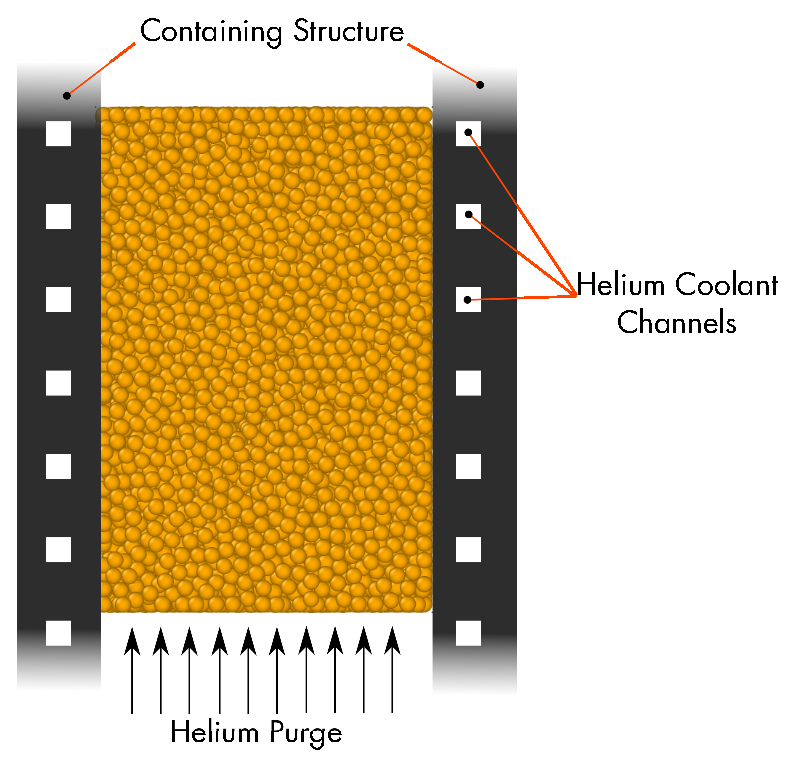
\includegraphics[width=0.85\textwidth]{chapters/figures/solid_breeder_sketch} 
	\caption{Sketch of a typical unit of a pebble bed tritium breeding zone. The pebble bed is cooled with contact to the containing structure.}
	\label{fig:solid-breeder-sketch}
\end{figure}
\end{frame}

\begin{frame}{Modeling Techniques}
\begin{block}{Discrete element method}
Particle-scale information of forces and temperatures for modeling and predicting pebble damage
\end{block}
\begin{block}{Coupled computational fluid dynamics and discrete element method}
Volume-averaging fluid flow for efficient simulations of large volumes with transient, coupled modeling to pebble-scale DEM computations
\end{block}
\begin{block}{Lattice-Boltzmann method}
Interrogate the entire, tortuous flow path with efficient modeling of fluid flow through geometrically complex packing structures
\end{block}
\end{frame}
\section[Lit. Review]{Literature Review}
\input{presentation/lit-review.tex}
\section[Model Dev.]{Development of Modeling Tools for Pebble Bed Morphological Evolution Studies}
\subsection{DEM Model}
\begin{frame}{Particle Dynamics}
\begin{columns}[t]
\column{.5\textwidth}
	Track particle trajectories,
	\begin{equation}
	\label{eq:newtons-second}
		m_i  \ddt{\vec{r}_i}  = m_i\vec{g} + \sum_{j=1}^{Z} \vec{f}_{n,ij} 
	\end{equation}

	\begin{subequations}
	\begin{align}
		\vec{f}_{n,ij} &= k_{n,ij} \delta_{n,ij}\vec{n}_{ij} - \gamma_{n,ij} \vec{u}_{n,ij} 	\label{eq:normal-force} \\
		k_{n,ij} &= \frac{4}{3}E_{ij}^*\sqrt{R_{ij}^*\delta_{n,ij}}
	\end{align}
	\end{subequations}

	\begin{subequations}
	\begin{align}
		\frac{1}{R_{ij}^*} &= \frac{1}{R_i} + \frac{1}{R_j} \\
		\frac{1}{E_{ij}^*} &= \frac{1-\nu_i^2}{E_i} + \frac{1-\nu_j^2}{E_j}
	\end{align}
	\end{subequations}


\column{.5\textwidth}
	\begin{figure}
		\centering
		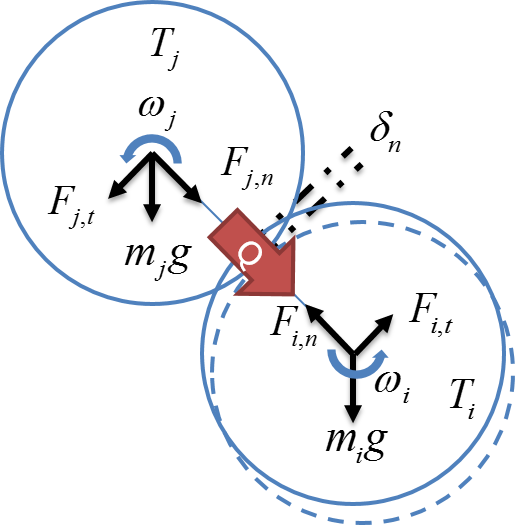
\includegraphics[width=0.5\linewidth]{chapters/figures/particle-interaction-drawing} 
		\caption{Allowing fictive overlap, $\delta$, between centroids to determine repulsive force between pebbles.}
		\label{fig:interacting-particles}
	\end{figure}
	 

	Equations of motion are integrated with the Velocity-Verlet algorithm -- global error of approximately $O(\Delta t^2)$

\end{columns}




\end{frame}

%~~~~~~~~~~~~~~~~~~~~~~~~~~~~~~~~~~~~~~~~~~~~~~~~~~~~~~~~~~~~~~~~~~~~~~~~~~~~~~~~~~~~~~~~~~~~~~~~~~~

% \begin{frame}
% Velocity-Verlet time integration
% \begin{subequations}
% \begin{align}
% 	\vec{a}_t &= \vec{g} + \frac{\vec{f}_t}{m}\\
% 	\vec{r}_{t+\Delta t} &= \vec{r}_t + \vec{v}_t\Delta t + \frac{1}{2}\vec{a}_t\Delta t^2\\
% 	\vec{v}_{t+\Delta t} &= \vec{v}_t + \frac{\vec{a}_t + \vec{a}_{t+\Delta t}}{2}\Delta t
% \end{align}
% \end{subequations}
% \end{frame}

%~~~~~~~~~~~~~~~~~~~~~~~~~~~~~~~~~~~~~~~~~~~~~~~~~~~~~~~~~~~~~~~~~~~~~~~~~~~~~~~~~~~~~~~~~~~~~~~~~~~

\begin{frame}{Particle Heat Transfer}
\begin{equation}\label{eq:thermoFirstLaw}
	m_iC_i\ddt{T_i} = Q_{s,i} + \sum_{j=1}^Z H_c(T_i - T_j)
\end{equation}
\begin{equation}\label{eq:dem-conductance}
	H_c= 2k^*\left[\frac{3F_{n,ij}R^*}{4E^*}\right]^{1/3}
\end{equation}
\begin{equation}
	d_{p,i} = d_{p_0,i}\left[1+\beta_i\left(T_i - T_\text{ref}\right)\right]
\end{equation}
\end{frame}

%~~~~~~~~~~~~~~~~~~~~~~~~~~~~~~~~~~~~~~~~~~~~~~~~~~~~~~~~~~~~~~~~~~~~~~~~~~~~~~~~~~~~~~~~~~~~~~~~~~~

\subsection{CFD-DEM Model}
\begin{frame}{Particle in Fluid Field}
% \begin{figure}
% 	\centering
% 	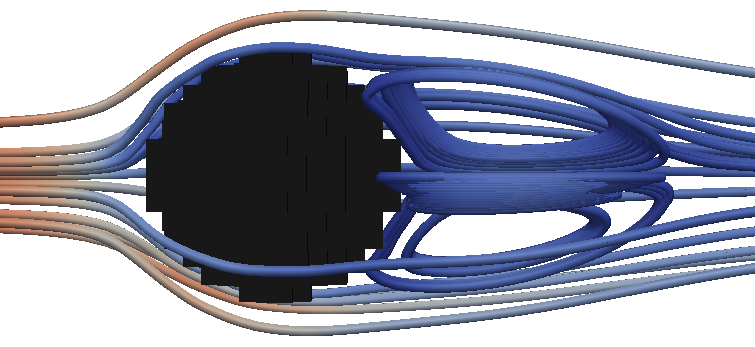
\includegraphics[width=0.5\linewidth]{chapters/figures/single-sphere-drag} 
% 	\caption{Streamlines around a single sphere in $Re = 100$ flow.}
% 	\label{fig:fluid-around-particle}
% \end{figure}

Add a drag on particle due to passing fluid and energy exchange at the interface. Eqs.~\ref{eq:newtons-second} and~\ref{eq:thermoFirstLaw} become,
\begin{subequations}\label{eq:cfdem-dem-momentum}
\begin{align}
	m_i  \ddt{\vec{r}_i}  &= m_i\vec{g} + \sum_{j=1}^{Z} \vec{f}_{n,ij} + \beta_i V_i \Delta \vec{u}_{if}\\
	m_iC_i \ddt{T_i} &= Q_{s,i} + \sum_{j=1}^Z Q_{ij} + \beta_{E,i} A_i \Delta T_{if}
\end{align}
\end{subequations}
the inter-phase exchange coefficients are defined as
\begin{subequations}
\begin{align}
	\beta_{i} &= \frac{18\mu_f}{d_{p,i}^2}(1-\phi_k)\phi_k F\\
	\beta_{E,i} &= \frac{\Nu k_f}{d_{p,i}}
\end{align}
\end{subequations}

\end{frame}


\begin{frame}{Non-dimensional Drag Correlations}
Koch, Hill, \& Ladd provide non-dimensional drag as
\begin{equation}\label{eq:khl-correlation}
	F = F_0(\phi) + F_3(\phi)\Re
\end{equation}
where 
\begin{subequations}
\begin{align}
F_0 &= \begin{cases}
	\frac{1+3(\phi/2)^{1/2} + (135/64)\phi\ln\phi + 16.14\phi}{1 + 0.681\phi - 8.48 \phi^2 + 8.16\phi^3} & \text{if $\phi < 0.4$}\\
	10.0\,\frac{\phi}{(1-\phi)^3} & \text{if $\phi > 0.4$} 
	\end{cases}\\
F_3 &= 0.0673 + 0.212\phi + 0.0232 \frac{1}{(1-\phi)^5}
\end{align}
\end{subequations}

Li \& Mason provide Nusselt number as
\begin{equation}\label{eq:li-mason-correlation}
	\Nu = \begin{cases}
	2+ 0.6\epsilon^n\Re_p^{1/2}\Pr^{1/3} 										& \Re_p < 200\\
	2+ 0.5\epsilon^n\Re_p^{1/2}\Pr^{1/3} + 0.02 \epsilon^n \Re_p^{0.8}\Pr^{1/3} & 200 < \Re_p < 1500\\
	2+ 0.000045\epsilon^n\Re_p^{1/2}			 								& \Re_p > 1500
	\end{cases}
\end{equation}
where they found from experiments that $n=3.5$ was appropriate for 3~mm polymer pellets in dilute flows
\end{frame}


\begin{frame}{Fluid Conservation Equations}
Volume-averaged Navier-Stokes and Energy equations with closure terms from DEM data,
\begin{subequations}\label{eq:cfd-equations}
\begin{align}
\pder[\epsilon_k \rho_f]{t} + \nabla\cdot(\epsilon_k \vec{u}_f \rho_f) &= 0\\
\pder[\epsilon_k \vec{u}_f]{t} + \nabla\cdot(\epsilon_k \vec{u}_f \vec{u}_f) &= -\frac{\epsilon_k}{\rho_f}\nabla P_f + \nabla\cdot\left(\nu_f\epsilon_k\nabla \vec{u}_f\right) - \frac{\vec{S}_k}{\rho_f}\\
\pder[\epsilon_k T_f]{t} + \nabla\cdot(\epsilon_k \vec{u}_f T_f) &= \nabla\left(\epsilon_k\nabla T_f\right)-\frac{E_k}{\rho_fC_f}
\end{align}
\end{subequations}

Coupling the fluid phase to the particles happens with the sink terms in momentum and energy of $\vec{S}_k$ and $E_k$
\begin{subequations}\label{eq:cfd-sources}
\begin{align}
	\phi_k &= 1- \epsilon_k = \frac{1}{V_k}\sum_{\forall i \in k} V_{p,i}\\
	\vec{S}_k &= \frac{1}{V_k}\sum_{\forall i \in k} \beta_i V_i \Delta \vec{u}_{if} \label{eq:cfd-mom-source}\\
	E_k &= \frac{1}{V_k}\sum_{\forall i \in k} \beta_{E,i} A_i \Delta T_{if}
\end{align}
\end{subequations}
\end{frame}

\begin{frame}{Lagrangian-Eulerian Mapping}
\begin{figure}[t]
	\centering
	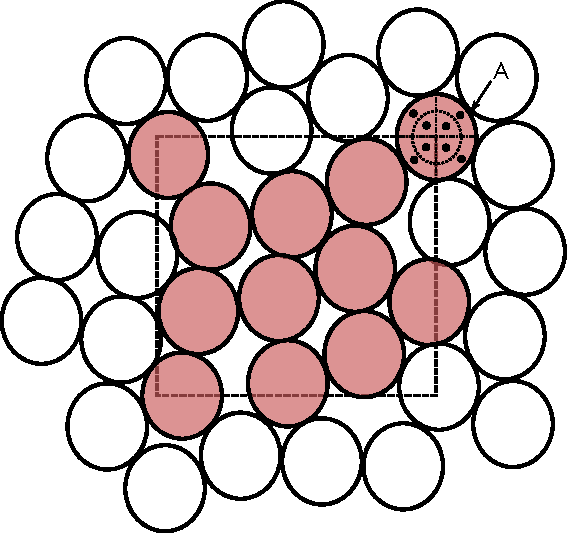
\includegraphics[width=0.5\linewidth]{chapters/figures/void-fraction-divided-cell.pdf}\label{fig:centroid-void-fraction-divided}
	\caption{The dashed line represents a computational cell in which exist many particles. The particles with centroids inside the cell are shaded red.}
\end{figure}
\begin{equation}
	\epsilon_\text{cell} = 1-\frac{1}{V_\text{cell}}\sum_{i = A}^{i=L}w_iV_{p,i}
\end{equation}
\end{frame}
\subsection{LBM}
\begin{frame}{Bhatnagar-Gross-Krook lattice-Boltzmann Formulation}
\begin{align}
	\underbrace{f_i(\vec{x}+\vec{c}_i, t + 1)  = f_i(\vec{x},t)}_\text{streaming}  + \underbrace{\Omega_i(\vec{x},t)}_\text{collision}
\end{align}

The collision operator is calculated based only on each nodes local information. Using the single-relaxation time BGK approximation the collision is calculated as
\begin{align}
	\Omega_i = -\frac{1}{\tau}\left[f_i(\vec{x},t) - f_i^\eq(\vec{x},t)\right]
\end{align}
Relaxation towards the equilibrium distribution function
\begin{equation}\label{eq:equilib-dist-function}
	f_i^\eq = \rho(\vec{x},t)w_i\left[1+\frac{\vec{u}\cdot\vec{c}_i}{c_s^2} + \frac{(\vec{u}\cdot\vec{c}_i)^2}{2c_s^4} - \frac{\vec{u}^2}{2c_s^2} \right]
\end{equation}

\end{frame}

\begin{frame}
Bounce-back boundary condition
\begin{figure}[t]
	\centering
	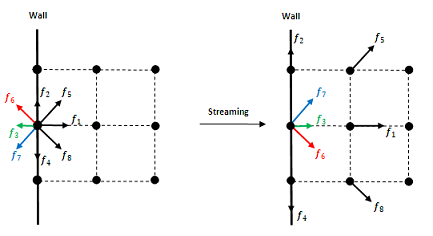
\includegraphics[width=0.5\linewidth]{chapters/figures/lbm/ongrid}\label{fig:wall-lattice-bc}
	\caption{Sketch of the D2Q9 nodes showing at the boundary the distribution functions that would come from neighbors outside the boundary (at the wall) are unknown (drawing from correspondence with Dr. Bao, billbao@cims.nyu.edu).}
\end{figure}
\end{frame}
\section[Studies]{Studies of Pebble Bed Thermophysics, Mechanics, \&  Morphological Changes}
\chapter{Initial Results, Validation, \& Discussions}\label{sec:dem-studies}

This chapter demonstrates the usefulness of the numerical tools introduced in \cref{ch:modeling-development} in probing inter-particle contact information, pebble bed heat transfer, and bed morphology changes altering thermophysical properties. The DEM, CFD-DEM, and DEM-LBM tools are put to work examining representative volumes of pebble beds of ceramic breeders from fusion reactors. In almost all cases, the pebble bed volumes accommodate approximately \num{10000} pebbles. Typically, the bed is confined in one direction by two primitive, rigid walls that also are constant temperature boundaries to act as heat sinks. I also employ periodic boundary conditions to represent an infinite length in the given direction. The third direction is often in the gravity direction for which we have an adiabatic, primitve, and rigid roof and ceiling.

The first study considers the heat transfer in a pebble bed purely through contact conduction of grains in the ensemble. In this pebble bed, I employ DEM tools to apply a nuclear heating source and allow the bed to reach a thermal steady-state with the cooling walls. In such a way, an effective thermal conductivity of the bed is determinable. I then induce a fictitious pebble damaging method to the bed and check the changes to effective thermal conductivity. The DEM tools are used to then interrogate many micromechanical interactions in the pebble bed which we use to deduce the source of changes to the effective thermal conductivity.

In the second study, the same pebble bed is analyzed but this time the helium purge gas is included via the coupled CFD-DEM tools. I again induce some fictitious damage to the pebble bed and monitor changes to the thermophysical properties and their relationship to the cases when the helium purge gas was neglected. The study reveals important features of the helium influence on heat transfer in the bed.

In the third study, I take snapshots of two beds (a standard bed and a damaged one) and load them into LBM models. With lattice-Boltzmann it is possible to analyze the tortuous path of helium moving through the pebble bed and discover interesting features of the purge gas thermal interaction that was masked by the simplifications of the volume-average approach of CFD-DEM.



%%%%%%%%%%%%%%%%%%%%%%%%%%%%%%%%%%%%%%%%%%%%%%%%%%%%%%%%%%%%%%%%%%%%%%%%%%%%%%%%%%%%%%%%%%%%%%
\section{DEM Study on Effective Conductivity of Pebble Peds with Pebble Damage}\label{sec:dem-studies-effective-conductivity}
% The discrete element method (DEM) is used by many ceramic breeder researchers to model the interaction of individual pebbles in an ensemble in an effort to obtain a more detailed understanding of pebble beds than is possible with experimental measurements of effective properties. For example see Refs.~\cite{An20071393, Lu2000, Zhao2010, Gan:2010uq, Annabattula2012a, VanLew2014}.

% The discrete element method has been used for studies in a variety of fields for studying inter-particle forces and the homogeneously distributed force networks that arise in packed beds.\cite{Makse2000} 

The discrete element method has been used by researchers in the fusion community to attempt modeling crushing initiation and propagation\cite{Annabattula2012a, Zhao2012, Zhao2013}. They observed that a relatively few number of high-force networks, distributed throughout the bed supported the external mechanical loads. The even distribution of the force networks was used to defend the development of a probability-based predictor for crushing by Zhao\etal.\cite{Zhao2013} The basic premise is that probability distributions of strength curves for pebble crushing have been observed (see, for example crush loads of Ref.~\cite{Tsuchiya1998}). Then in DEM models, a probability distribution of inter-particle forces are also observed. Overlaying the two probabilities resulted in seemingly random locations of pebbles satisfying the damage criteria -- not strictly along the high-force chains running through packed beds.

To separate studies of crushing initiation from its downstream effects on mechanical and thermal properties, I make use of results of Zhao\etal~to create fictitiously damaged beds without consideration of the initiation of the damage. Zhao\etal~found that, with their predictive tool, pebbles are crushed in random locations. If this is the case, I may de-couple the task of predicting pebble damage (\textit{i.e.} finding the mechanical or thermal load that causes a pebble to fail) from the task of modeling the ramifications of pebble crushing. I am free to randomly assign pebble damage to mimic the random locations from predictions. This is how I will model pebble damage in this first model.

As far as modeling the fragmentation, I begin with an extreme assumption of pulverization of the particle -- a not entirely unrealistic assumption. Experiments on crushing single, brittle pebbles reveal that there are a number of failure modes.\cite{Wu2004} At one extreme, the pebble may simply crack and continue to hold a load for some time. At the other extreme, a pebble may crush practically into a dust. The damage method used in this study is an extension of that latter extreme. When a pebble in our simulation has been flagged for damage, it is completely removed from the ensemble. The remaining pebbles are allowed to rearrange to compensate for the lack of equilibrium on their contact forces due to the missing pebbles. In later models I will use the fragmentation approach as outlined in \cref{sec:failure-study}.

\subsection{DEM Study: Effective Conductivity with Pebble Damage}
\label{sec:dem-studies-effective-conductivity}
The discrete element method has been used for studies in a variety of fields for studying inter-particle forces and the homogeneously distributed force networks that arise in packed beds (for example, see Ref.~\cite{Makse2000}). The discrete element method was also used in the fusion community to attempt to model crushing initiation and propagation\cite{Annabattula2012a, Zhao2012, Zhao2013}. They too observed that a relatively few number of high-force networks, distributed throughout the bed supported the external mechanical loads. The even distribution of the force networks was used to defend the development of a probability-based predictor for crushing. We make use of the probability argument of Zhao\etal~for the current study\cite{Zhao2013}. Their basic premise is that probability distributions of strength curves for pebble crushing have been observed (see, for example crush loads of Ref.~\cite{Tsuchiya1998}). Then in DEM models, a probability distribution of inter-particle forces are also observed. Overlaying the two probabilities resulted in seemingly random locations of pebbles satisfying the damage criteria -- not strictly along the high-force chains running through packed beds.

We apply the theory of Zhao\etal~in the following manner. If pebbles are crushed in random locations, we may de-couple the task of predicting pebble damage (\textit{i.e.} finding the mechanical or thermal load that causes a pebble to fail) from the task of modeling the ramifications of pebble crushing. Experiments on crushing single, brittle pebbles reveal that there are a number of failure modes\cite{Wu2004}. At one end, the pebble may simply crack and continue to hold a load for some time. At the other extreme, a pebble may crush practically into a dust. We concern ourselves with the latter for this study. When a pebble in our simulation has been flagged for damage, we remove the pebble completely from the ensemble and then allow the remaining pebbles to rearrange to compensate for the lack of equilibrium on their contact forces. 

In our model, we begin with a starting point of a packed bed and then simply flag pebbles at random for crushing. The removal disrupts the meta-static state of the ensemble and the remaining pebbles re-settle due to gravity and the imbalance of contact forces. In reality, the ceramic pebbles generally break into just a few large pieces that remain in the system, a simulation attempting to model such a crush event is covered in \cref{sec:applied-studies}.

\subsubsection{Model Setup \& Methodology}\label{sec:dem-setup}
We analyze a three-dimensional pebble bed consisting of mono-dispersed particles of diameter $d_p$. The particles are constrained by rigid $y-z$-planes at locations of $\frac{x}{d_p} = \pm 10$ (the walls of our container). There are periodic boundary conditions in the $y$-direction located at $\frac{y}{d_p} = \pm 7.5$. Gravity acts in the negative $z$-direction and the particles are resting on a rigid $x-y$-plane at $z=0$ (the floor of the container) and held from the top by an $x-y$-plane at $\frac{z}{d_p} = 30$ (the roof of the container). We pack to $\phi = 64\%$ and, given the volume, have 11000 particles. The volume was chosen to represent the long, tall, narrow channels seen in many solid breeder module designs\cite{ Cho2008, Poitevin2010, Enoeda2003}.

For this study, the material properties were chosen to represent lithium metatinatate pebbles. All the properties come from Ref.~\cite{Gierszewski1998}. They are summarized in Table~\ref{tab:mat-props}

\begin {table}[tp] %
\caption{Maximum load and nominal tension.}
\label {tab:mat-props} \centering %
\begin {tabular}{ cccccc }
\toprule %
E           &     $\nu$    	&    k         	&    C          &   $\alpha$                \\
(GPa)    	&            	& (W/m-K) 		&  (J/kg-K)  	&   (1/K)                   \\\toprule
126			&      0.24     &  2.5          &  1156       	&   $15\times10^{-6}$		\\\bottomrule
\end{tabular}
\end{table}

In the first attempt at packing pebbles into the system, we begin with a common starting point of a filled, lightly packed volume of 10~550 pebbles. We simulate pouring the pebbles into the volume by initializing them into the system from a height of $\frac{z}{d_p} \approx 50$ and allow them to fall under the influence of gravity (see Fig.~\ref{fig:fill01}). We pack the pebbles into a higher packing fraction by means of oscillating the walls as if the pebble bed were sitting on a vibrating plate. This was to imitate the vibration packing technique done in our experimental lab when testing pebble beds in the uniaxial compression test stand. The vibration scheme was able to slowly densify the packed bed but, owing to the very small timestep of the simulation, the simulation times were impractically large to approach a packing fraction greater than $\phi = 60\%$. 

\begin{figure}[!ht]
	\centering
	\begin{subfigure}[b]{0.25\textwidth}
		\centering
		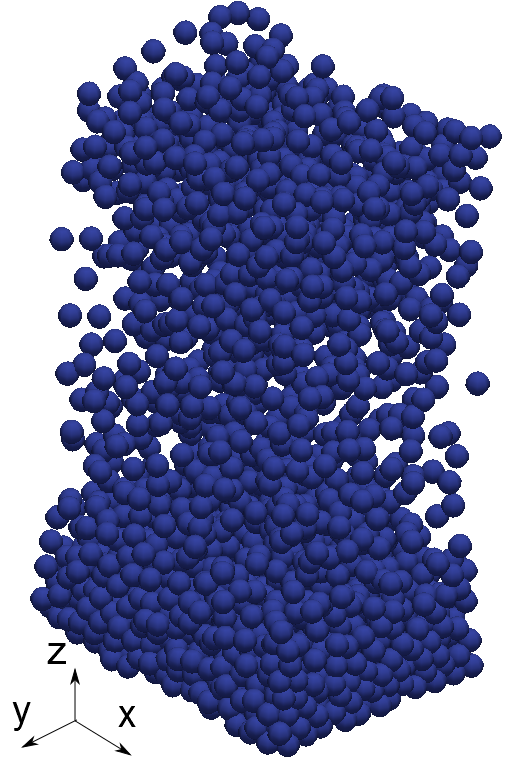
\includegraphics[width=\textwidth]{chapters/figures/fill01.png}
	\end{subfigure}
	\begin{subfigure}[b]{0.25\textwidth}
		\centering
		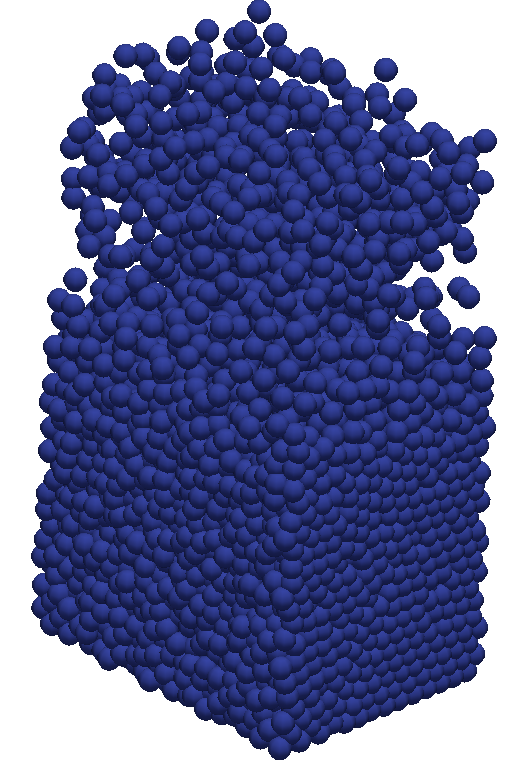
\includegraphics[width=\textwidth]{chapters/figures/fill02.png}
	\end{subfigure}
	\begin{subfigure}[b]{0.25\textwidth}
		\centering
		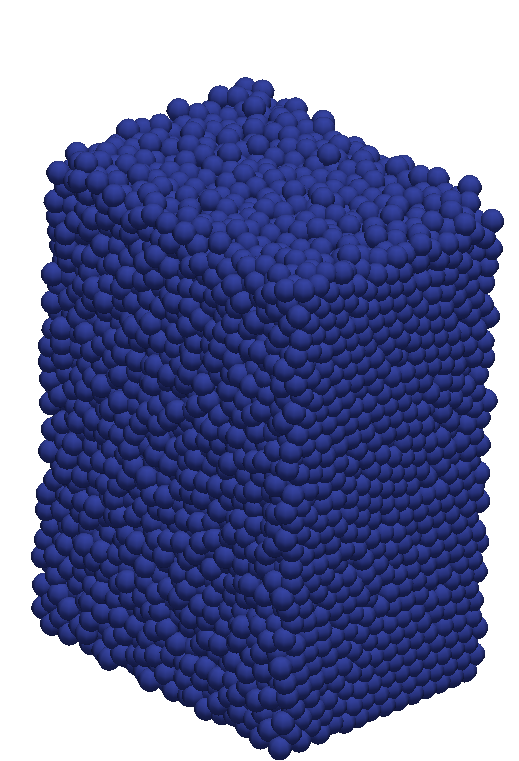
\includegraphics[width=\textwidth]{chapters/figures/fill03.png}
	\end{subfigure}
	\caption{Demonstrating the pouring process of $N = 10550$ pebbles into the control volume with at an early time (left), when it is nearly filled (middle) and after the pebbles have settled to negligible kinetic energy (right).}
\label{fig:fill01}
\end{figure}

In the end, a simpler pack-relax method was used instead. In this method $N$ particles are inserted into the volume such that we have precisely the packing fraction we desire (in this case, $\phi = 64\%$ so $N = 11000$). The pebbles are placed at random into the volume and are allowed to artificially overlap -- often by a great deal ($\delta \sim R_p$). The overlap they experience would normally cause such an enormous force (integrating into an enormous velocity) that the pebbles would all explode out of the bed at the first step in time integration. We avoid such a catostrophic scenario with a relaxation scheme where we truncate the displacement of any pebble per timestep that is integrated from the force. The truncated displacement is very small and allows the pebbles to slowly move away from each other and into a static equilibirum as the artifical overlap is reduced. Once the pebble bed comes to rest, we remove the relaxation (limiting displacement command) and allow standard integration of contact forces with the velocity-Verlet algorithm (see \cref{sec:velocity-verlet}). The pack-relax scheme allowed for obtaining desireable, highly repeatable packing fractions for all pebble beds. Once the pebble bed was packed into an initial condition, the simulation state was saved and used as a starting point for the numerous `crushed' cases to be described later.

In this first study, we model pebble crushing without considering why the particular pebble should be cracking. In the model we randomly select pebbles from the ensemble, regardless of forces acting upon the pebble, and delete them entirely from the system. When a pebble is removed, the neighboring pebbles react due to the imbalance of forces, and the bed settles into a new configuration. We differentiated the failed beds by their percentage of failed pebbles: $\eta = $ number of failed pebbles per original ensemble size. For the baseline case and for beds after failing, we apply the heating routine described next.

To simulate the conditions of a solid breeder in a fusion reactor, where the heat is removed from the pebble bed via contact to the containing structure, we assigned a constant temperature of $T_\text{c}$ to the vertical walls. Nuclear heating of the pebbles is simulated through a constant source term on each pebble. A representative heating rate of $Q_s = q_p'''V_p$, where  $q_p'''= 8$ MW/m$^3$. The heating cycle runs until a thermal steady state is reached. Based on a measurement of the total thermal energy of the bed, $E_T =\sum_i^N m_iC_i T_i$, steady-state is determined as $\dt{E_T} = 0$ within a specified tolerance. Once at steady state, we analyzed thermal and mechanical characteristics of the pebble bed: effective thermal conductivity, average coordination number, temperature profiles in the bed, and inter-particle contact forces. 

Based on the boundary conditions to our system, we establish heat transfer that is symmetric and one-dimensional in the $x$-direction from $x=0$ to the walls at $\frac{x}{d_p} = \pm 10$. As we will show, the pebble bed has very little variation of forces and temperatures in the $y$-direction due to the periodic boundary condition at the edges of the domain. Gravity effects are minor in the overall heat transfer and induce only a slight $z$-dependency to the results. We take advantage of this nature of our pebble bed to find the effective conductivity from an analytic, one-dimensional test case.
%~~~~~~~~~~~~~~~~~~~~~~~~~~~~~~~~~~~~~~~~~~~~~~~~~~~~~~~~~~~~~~~~~~~~~~





%~~~~~~~~~~~~~~~~~~~~~~~~~~~~~~~~~~~~~~~~~~~~~~~~~~~~~~~~~~~~~~~~~~~~~~
\subsubsection{Effective Thermal Conductivity from Analytic Analogy}
Assuming a one-dimensional pebble bed, to find an effective conductivity, we step back into a continuum mechanics formulation where the pebble bed can be represented as a slab of solid material. We can analytically solve for the temperature equation in a slab with heat generation, symmetry about the centerline, and a constant boundary temperature condition.

At steady-state, the temperature of a material with constant temperature boundary conditions ($T(L) = T_s$), constant thermal conductivity ($k_\text{eff}$), and nuclear heating ($q'''$) obeys the following equation

\begin{equation}\label{eq:continuum-heateqn}
	0 = \frac{\mathrm{d}^2T}{\mathrm{d}x^2} + \frac{q'''}{k_\text{eff}}
\end{equation}

We introduce a non-dimensional temperature
\begin{equation}
	\theta = \frac{T(x) - T_s}{T_0 - T_s}
\end{equation}
where $T_0$ is the temperature at the centerline of this slab (a value we will find momentarily). The length is non-dimensionalized as
\begin{equation}
	x^* = \frac{x}{L}
\end{equation}

Thus we can re-write Eq.~\ref{eq:continuum-heateqn} as
\begin{equation}\label{eq:continuum-heateqn-nondim}
	0 = \frac{\mathrm{d}^2\theta}{\mathrm{d}x^{*2}} + G
\end{equation}
where
\begin{equation}
	G = \frac{q'''L^2}{k_\text{eff}(T_0 - T_s)}
\end{equation}

In the non-dimensionalized form, the solution is revealed to be purely geometric,
\begin{equation}\label{eq:continuum-temperature-nondim}
	\theta = 1-x^{*2}
\end{equation}. 
as $T_0  - T_s = \frac{q'''L^2}{2k_\text{eff}}$. We will use the non-dimensional temperature solution of Eq.~\ref{eq:continuum-temperature-nondim} to prove our one-dimensional assumption of heat transfer is justified for the pebble beds.

We note that in this continuum mechanics formulation, we are assuming that the nuclear source, $q'''$ term is applied evenly over the entire volume. In our DEM formulation, our source term applies to a single pebble. To find the effective thermal conductivity of our `slab' of pebble bed, we must reconcile this discrepency. This is accomplished with the exchange of
\begin{equation}\label{eq:q-source-translation}
	q''' = \frac{Q_\text{tot}}{V_\text{tot}} = \frac{Q_sN}{H\cdot L\cdot W\cdot d_p^2}
\end{equation}
where the pebble bed volume is given by the height, $H$, width, $W$, and length, $L$, and $Q_s$ is the source term on each pebble in the DEM ensemble. 

From the solution of Eq.~\ref{eq:continuum-heateqn-nondim}, we find the effective conductivity to be
\begin{equation}
	k_\text{eff} = \frac{q''' L^2}{2(T_0-T_s)}
\end{equation}
and when we replace the heat generation term with Eq.~\ref{eq:q-source-translation}, and use the bed dimensions as given in \cref{sec:dem-setup}, this is written as
\begin{equation}\label{eq:dem-effecitve-conductivity-formula}
	k_\text{eff} = \frac{Q_sN}{180(T_0-T_s)d_p}
\end{equation}

We will use this formulation of Eq.~\ref{eq:dem-effecitve-conductivity-formula} to analyze and compare the pebble beds of this study.
% \begin{figure}[htbp]
% 	\centering
% 	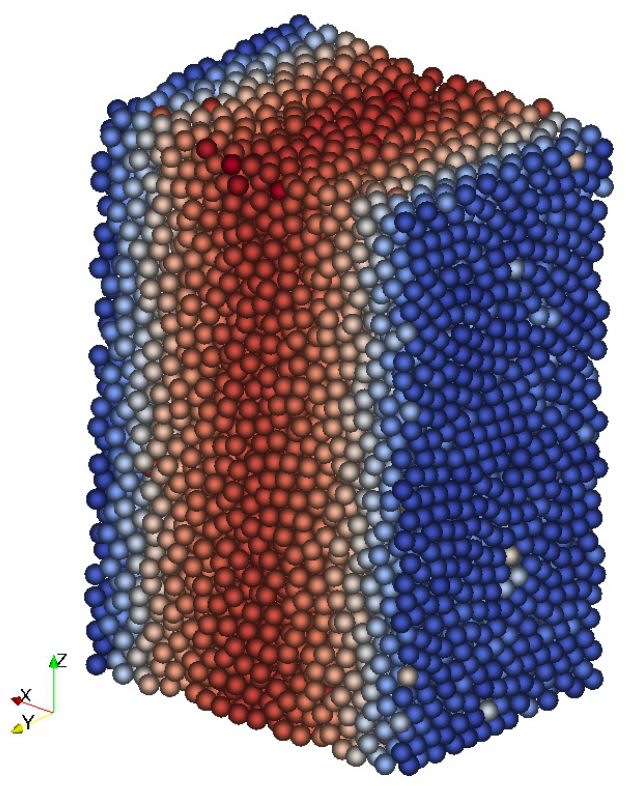
\includegraphics[trim=1cm 8cm 3cm 4cm, width=0.5\textwidth]{chapters/figures/pebbleBedTemperature}
% 	\caption{Temperature distribution of pebbles in the $10\%$ failed bed. At the end of steady-state heating, a one-dimensional profile is evident in all pebble beds studied here. The pebbles are receiving nuclear heating. Cooling proceeds through the pebbles in contact with the walls in the $x$-direction.}
% \label{fig:pebbleBedTemperature}
% \end{figure}



\subsubsection{Results}
The aim of this study was both to discover the impact of pebble failure on thermo-mechanical properties as well as determine the impact as a function of the number of failed pebbles. To satisfy the latter, we created beds with $\eta = 1\%$, $3\%$, $5\%$, $10\%$, and $15\%$ of pebbles failed. 

We plot Eq.~\ref{eq:continuum-temperature-nondim} against the non-dimensionalized temperature profiles coming from the steady-state DEM simulation in Fig.~\ref{fig:temp-scatters}. We find that all our models had a nearly perfect match to a one-dimensional prediction, validating the calculation of effective thermal conductivity in this study. Furthmore, the profiles adhering to the one-dimensional curve also allows us to find the effective conductivity of each bed from applying Eq.~\ref{eq:dem-effecitve-conductivity-formula}, which was derived from the one-dimensional assumption.

One concern we had for pebble crushing, was the phenomenon of `jamming' during resettling that would possibly leave pebbles isolated from their neighbors (apart from those they are resting upon). Jamming can happen when a bridge of pebbles have a balance for forces without strong or any contact to a pebble below them. The pebble under the bridge then only has light contact with the pebbles upon which it is resting. Such an isolated pebble would have no strong pathway for heat transfer and heat up much higher than that of its neighbors. Evidence of pebble isolation is apparent in hot individual pebbles above the grouped curve in Fig.~\ref{fig:temp-scatters}. 

\begin{figure}[htbp]
	\centering
	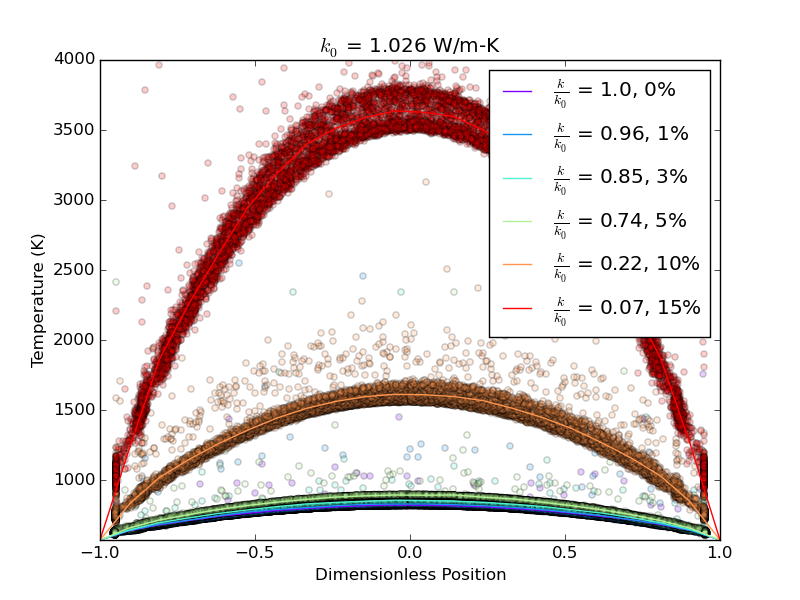
\includegraphics[width=0.65\textwidth]{chapters/figures/dem-evap-0-15-scatter-keff.png}
	\caption{The nondimensional temperature profiles for each test case follow the theoretical shape of a one-dimensional, constant $k$, continuum solution.}
\label{fig:temp-scatters}
\end{figure}

Because the 10\% and 15\% cases have such high temperatures, we show only the 0-5\% crushed together in Fig.~\ref{fig:temp-scatters-zoomed}

\begin{figure}[htbp]
	\centering
	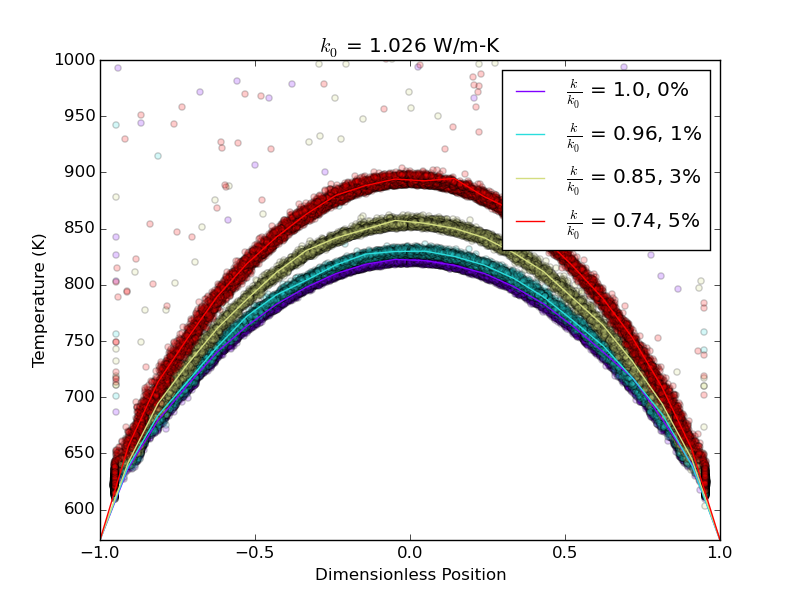
\includegraphics[width=0.65\textwidth]{chapters/figures/dem-evap-0-5-scatter-keff.png}
	\caption{The nondimensional temperature profiles for the test cases up to 5\% crushed pebbles.}
\label{fig:temp-scatters-zoomed}
\end{figure}

The individual hot pebbles in Fig.~\ref{fig:temp-scatters} are also indicative of the shortcomings of the discrete element method for modeling solid breeders in fusion reactors. The flowing purge gas in actual solid breeders would likely not permit such thermal isolation of pebbles. Even if a pebble had no physical contact with neighboring ones, it would still transport energy via conduction and advection of the helium gas. This will be addressed again and in more detail in \cref{sec:cfd-dem-effective-conductivity}.

In order to calculate an effective conductivity of the pebble bed, we must find an average temperature profile through the bed to compare with Eq.~\ref{eq:continuum-temperature-nondim} and thus employ Eq.~\ref{eq:dem-effecitve-conductivity-formula}. We compare steady-state temperature profiles in the test beds against the one-dimensional, non-dimensional temperature profile. Average values of the bed, along the $x$ direction, are generated via averaging temperatures in bins. We create bins that are volumes slices of width $\Delta x$ that extend through the limits of the $y$- and $z$-directions. We then find the $n$ pebbles residing in the slices and take the mean value of their temperatures. The average, given by Eq.~\ref{eq:binned-T}, is also given in Fig.~\ref{fig:temp-scatters}. The binned average temperature is 
\begin{equation}\label{eq:binned-T}
	\langle T\rangle = \frac{1}{n}\sum_{i}^n T_i 	
\end{equation}
Using the volume slices, we also find the average coordination number, 
\begin{equation}\label{eq:binned-z}
	\langle Z \rangle = \frac{1}{n}\sum_{i}^n Z_i
\end{equation}
and average contact force, 
\begin{equation}\label{eq:binned-f}
	\langle F^{1/3} \rangle = \frac{1}{n}\sum_{i}^n F_{n,ij}^{1/3}
\end{equation}


In Eq.~\ref{eq:thermoFirstLaw} of \cref{sec:dem-heat-transfer}, we see that at steady-state, the energy input by nuclear heating must be balanced by the transport of heat out of a pebble into its neighbors. Inter-particle heat transfer is dictated by the number of neighboring contacts, temperature difference between pebbles, and the thermal conductance, $H_{c}$, through the contact area. The thermal conductance (see Eq.~\ref{eq:dem-conductance}) is itself a function purely of material properties  (which are essentially constant here) and the force at the contact, going as $H_{c} \propto F_{n,ij}^{1/3}$. Thus, we write the net heat out of a pebble at steady state as a function of the three variables,

\begin{equation}
	Q_\text{net} =f( Z, F_n^{1/3}, \Delta T)
\end{equation}

The coordination number and contact forces are features of the packing structure in the packed bed that we can analyze to discover what happens to the heat flux between pebbles when the bed experiences crushed particles. Conversely, the $\Delta T$ between two pebbles is the effect of the thermal transport (i.e. leading to higher bed temperatures such as those of Fig.~\ref{fig:temp-scatters}). We will first analyze the changes to the coordination numbers of pebbles in the ensemble as pebbles crush.


\begin{figure}[!ht]
	\centering
	\begin{subfigure}[b]{\doubleimagewidth}
		\centering
		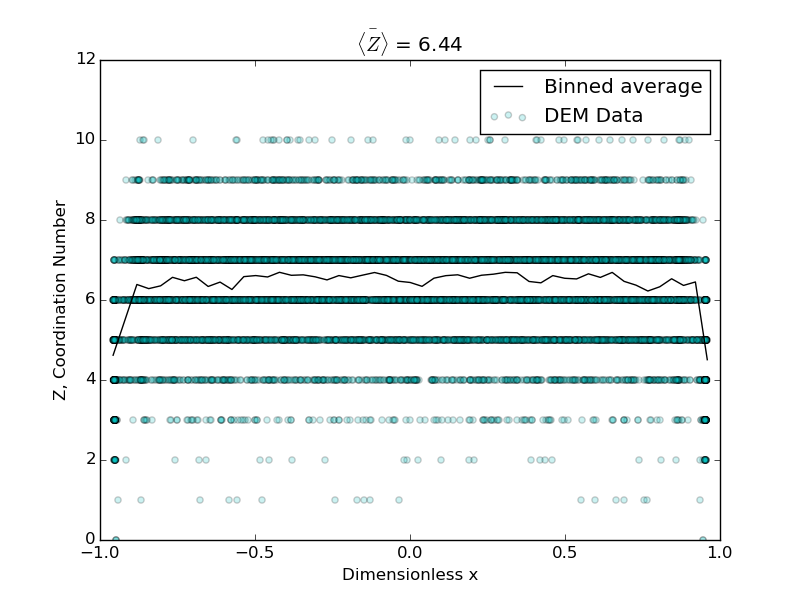
\includegraphics[width=\textwidth]{chapters/figures/heating_dte-02/dem-evap-0-scatter-coord.png}
		\caption{Baseline pebble bed (0\% crushed)}
	\end{subfigure}
	\begin{subfigure}[b]{\doubleimagewidth}
		\centering
		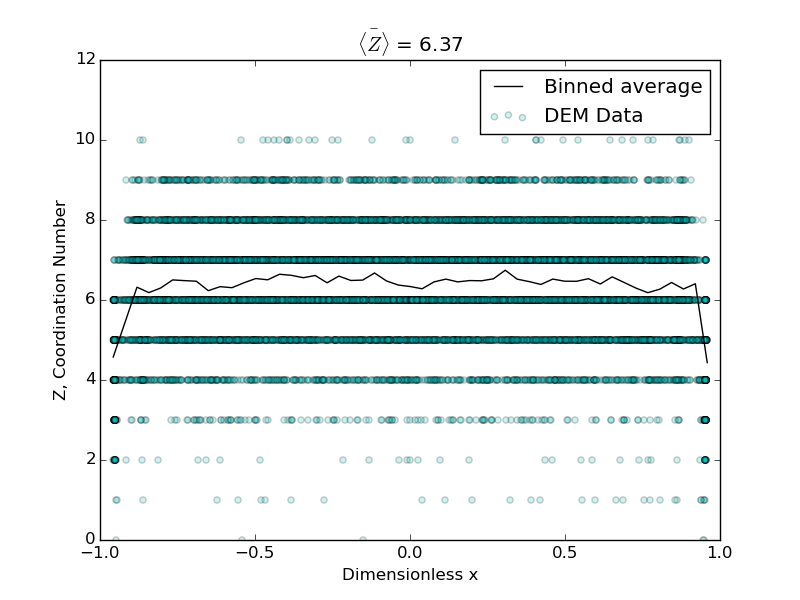
\includegraphics[width=\textwidth]{chapters/figures/heating_dte-02/dem-evap-1-scatter-coord.png}
		\caption{1\% crushed}
	\end{subfigure}
	
	\begin{subfigure}[b]{\doubleimagewidth}
		\centering
		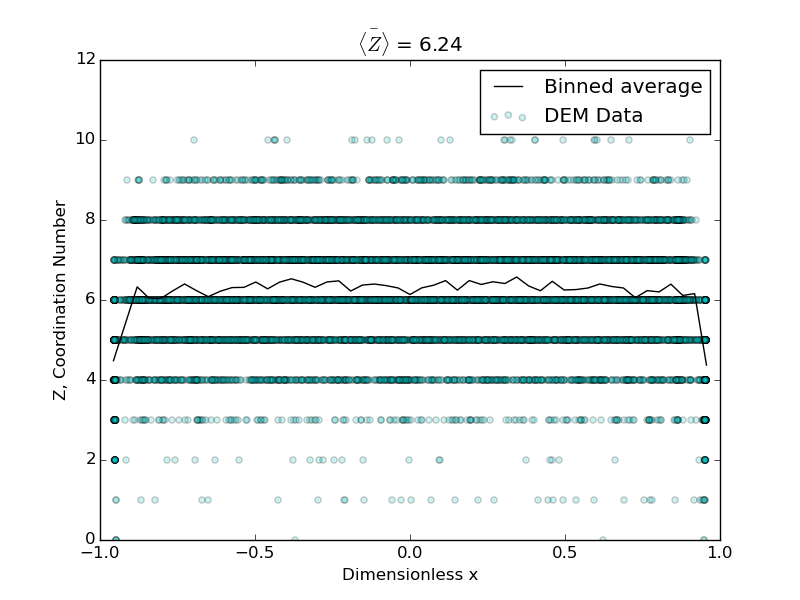
\includegraphics[width=\textwidth]{chapters/figures/heating_dte-02/dem-evap-2-scatter-coord.png}
		\caption{3\% crushed}
	\end{subfigure}
	\begin{subfigure}[b]{\doubleimagewidth}
		\centering
		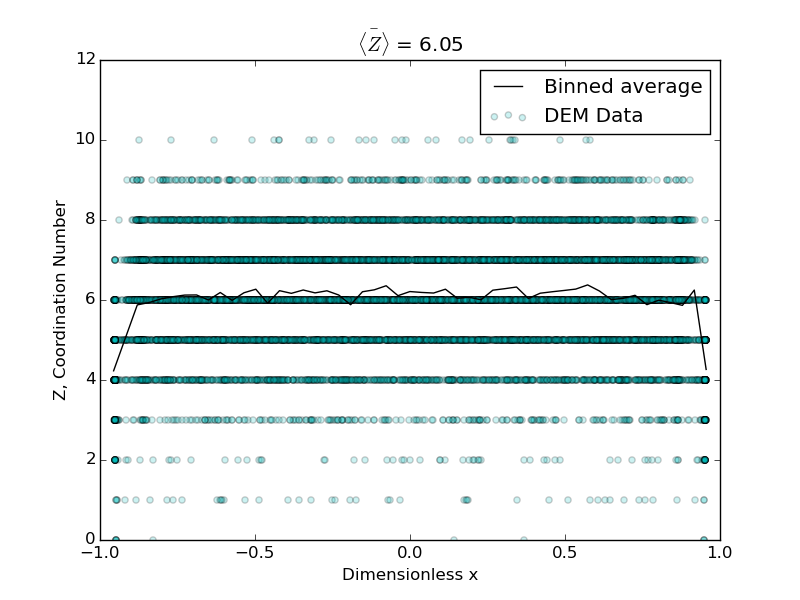
\includegraphics[width=\textwidth]{chapters/figures/heating_dte-02/dem-evap-3-scatter-coord.png}
		\caption{5\% crushed}
	\end{subfigure}

	\begin{subfigure}[b]{\doubleimagewidth}
		\centering
		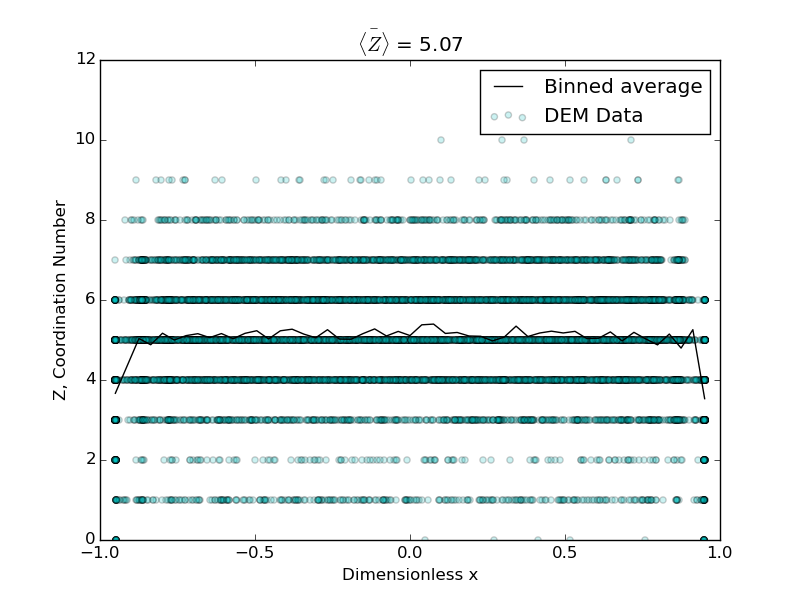
\includegraphics[width=\textwidth]{chapters/figures/heating_dte-02/dem-evap-4-scatter-coord.png}
		\caption{10\% crushed}
	\end{subfigure}
	\begin{subfigure}[b]{\doubleimagewidth}
		\centering
		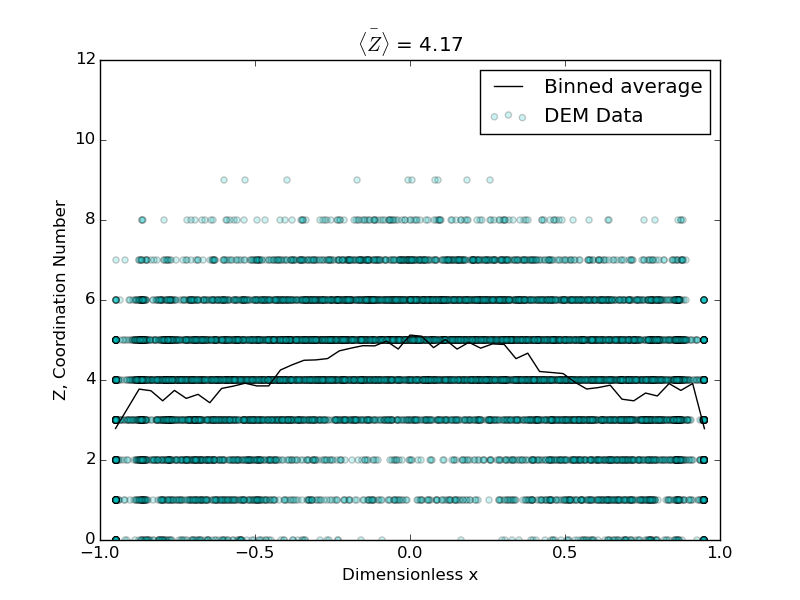
\includegraphics[width=\textwidth]{chapters/figures/heating_dte-02/dem-evap-5-scatter-coord.png}
		\caption{15\% crushed}\label{fig:coord-scatter-15percent}
	\end{subfigure}
	\caption{The average coordination number decreases slowly as the number of broken pebbles in the ensemble increases.}
\label{fig:coord-scatter}
\end{figure}

In Fig.~\ref{fig:coord-scatter} we plot the data for all pebbles in the ensemble as well as the binned average (Eq.~\ref{eq:binned-z}). Clearly, there are fewer average contacts per pebble in the ensemble after failure; At 15\% crushed the coordination number drops by roughly 30\%. But this alone can not not account for the reduction in $k_\text{eff}$ by 93\% for the same amount of crushed pebbles. Next we look to the normal contact forces between pebbles in the bed.


\begin{figure}[!ht]
	\centering
	\begin{subfigure}[b]{0.4\textwidth}
		\centering
		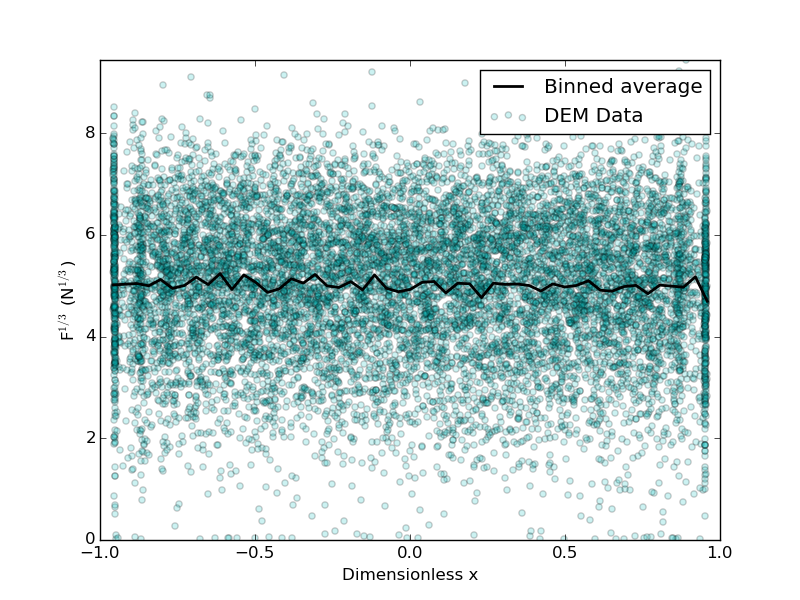
\includegraphics[width=\textwidth]{chapters/figures/heating_dte-02/0/dump/force-profile.png}
		\caption{Baseline pebble bed (0\% crushed)}
	\end{subfigure}
	\begin{subfigure}[b]{0.4\textwidth}
		\centering
		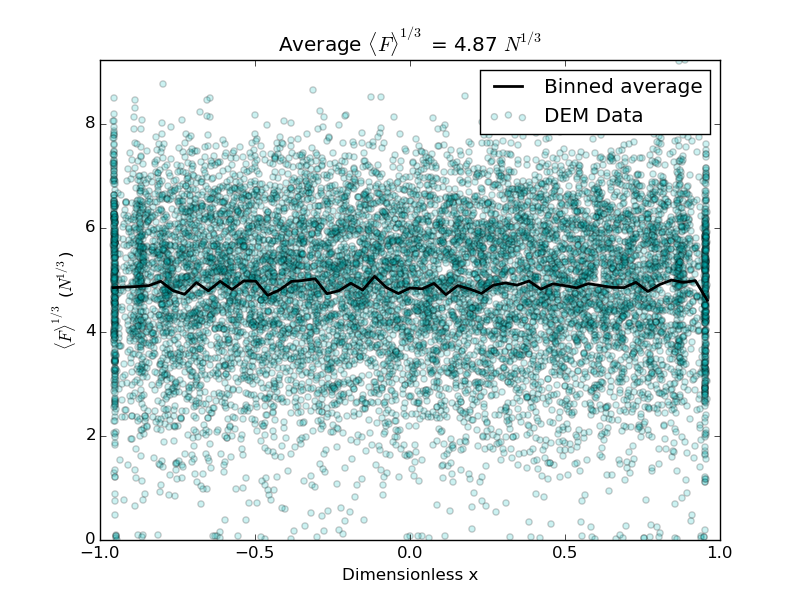
\includegraphics[width=\textwidth]{chapters/figures/heating_dte-02/1/dump/force-profile.png}
		\caption{1\% crushed}
	\end{subfigure}
	
	\begin{subfigure}[b]{0.4\textwidth}
		\centering
		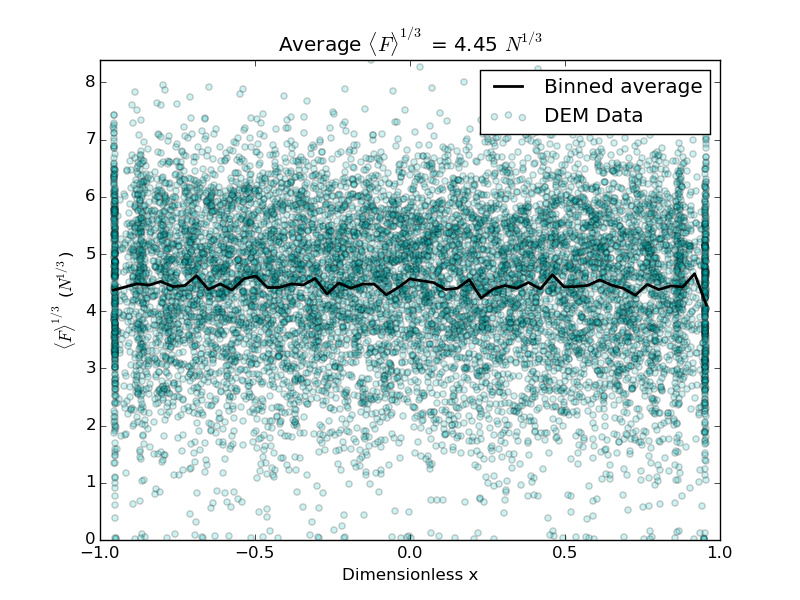
\includegraphics[width=\textwidth]{chapters/figures/heating_dte-02/3/dump/force-profile.png}
		\caption{3\% crushed}
	\end{subfigure}
	\begin{subfigure}[b]{0.4\textwidth}
		\centering
		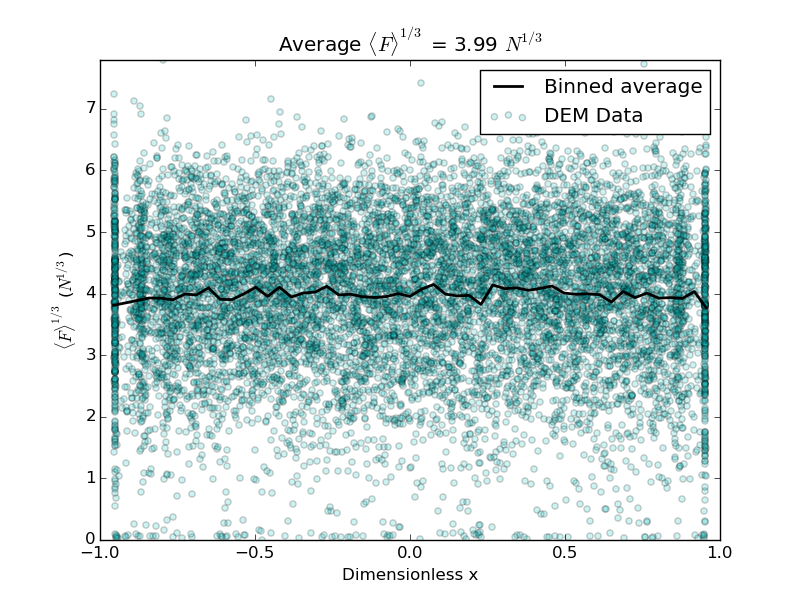
\includegraphics[width=\textwidth]{chapters/figures/heating_dte-02/5/dump/force-profile.png}
		\caption{5\% crushed}
	\end{subfigure}

	\begin{subfigure}[b]{0.4\textwidth}
		\centering
		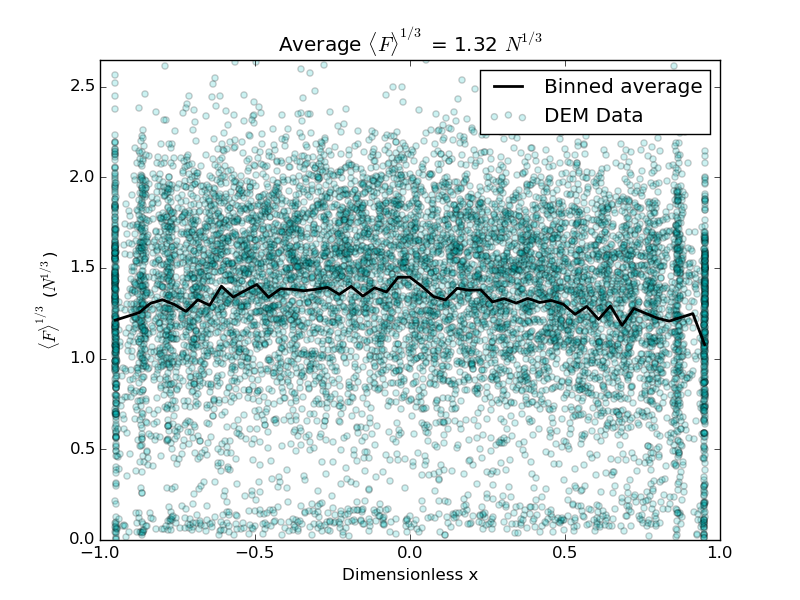
\includegraphics[width=\textwidth]{chapters/figures/heating_dte-02/10/dump/force-profile.png}
		\caption{10\% crushed}
	\end{subfigure}
	\begin{subfigure}[b]{0.4\textwidth}
		\centering
		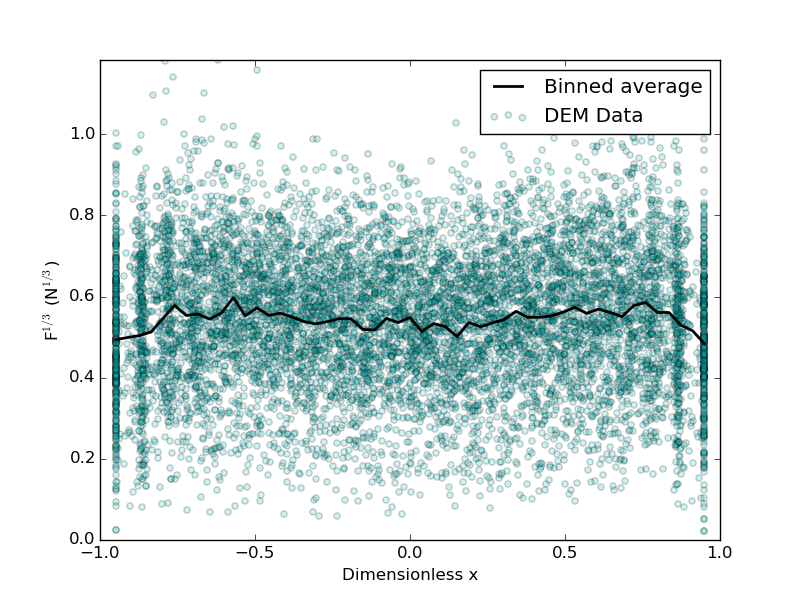
\includegraphics[width=\textwidth]{chapters/figures/heating_dte-02/15/dump/force-profile.png}
		\caption{15\% crushed}\label{fig:contact-forces-scatter-15percent}
	\end{subfigure}
	\caption{As pebble beds experience massive amounts of crushed pebbles (>5\%), the contact forces in the ensemble (after heating to steady-state) show dramatic reductions in value. Note the change of scale on the figures from the baseline case to the 15\% crushed case.}
\label{fig:contact-forces-scatter}
\end{figure}

The normal contact forces between pebbles are plotted in Fig.~\ref{fig:contact-forces-scatter}. A dramatic reduction in the normal forces is seen after many of their neighbors are crushed and are removed from the system. From the baseline down to the 15\% failed case, the contact forces are reduced by about a factor of 10 - similar to the reduction in effective conductivity.

The effective thermal conductivity was found for all of our pebble beds, via Eq.~\ref{eq:dem-effecitve-conductivity-formula}, then normalized against the conductivity of the baseline ensemble ($k^* = k/k_\text{0}$). The average coordination number of the beds and average normal contact forces were also found. Another way of describing a pebble bed is with the packing fraction, $\phi$. In Fig.~\ref{fig:packing-fraction}, we collect all these values (and normalize them against the baseline case) to provide a direct comparison to their changes as a function of crushed pebbles. When $15\%$ of the pebbles are crushed in a pebble bed, the effective conductivity has fallen all the way to only $k^*=0.07$. This large reduction is especially important in light of the already poor thermal management of virgin pebble beds that, even in helium environments, have been experimentally measured at only approximately 1~W/m-K (see, { e.g.}, Refs.~\cite{Reimann:2002mi, Piazza2002811}). The only parameter to have similar reductions in value is the average normal contact force, a value which is seen to follow closely to the curve of effective conductivity. Thus we conclude that the single most important factor for determining the effective thermal conductivity in these pebble beds is the normal contact forces between pebbles; a force which decreases sharply as pebbles are crushed in the system.

\begin{figure}[!ht]
	\centering
	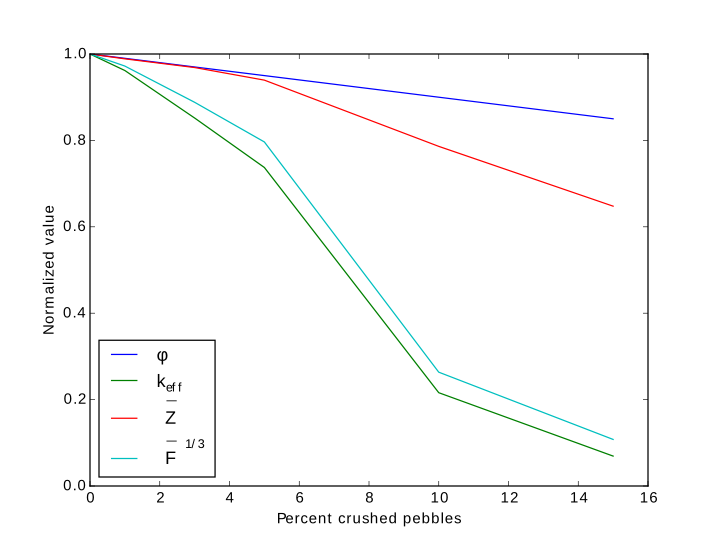
\includegraphics[width=\singleimagewidth]{chapters/figures/kEff_packingFraction}
	\caption{The normalized effective conductivity drops much more rapidly than the normalized packing fraction, $\phi$, while pebbles are crushed. The effective conductivity follows with reduced normal contact forces.}
\label{fig:packing-fraction}
\end{figure}

The large reduction in normal contact force (which leads to a large reduction in effective conductivity) is explainable based on the experimental setup of our numeric model. In our system, we had rigid walls in the $x$ and $z$ directions. These walls did not change after the substantial number of pebbles were crushed and removed. After the 15\% crushing event, the pebble bed appeared as Fig.~\ref{fig:15percent-crushed-pre}. A massive re-arrangement proceeds from the crushing event. As the pebble bed heats up, the thermal expansion of the pebbles is unconstrained as there exists an average of two pebble diameter gap above the pebbles to the top of the container. Numerically there is no limit to the pebble temperatures (phase change and sintering is not incorporated into the DEM calculations) so the pebbles heat and swell until coming into contact with the top wall, at which time they begin to press into one another (though lightly) to allow thermal conduction. The pebble bed after swelling is shown in Fig.~\ref{fig:15percent-crushed-swelling}.

\begin{figure}[!ht]
	\centering
	\begin{subfigure}[t]{\doubleimagewidth}
		\centering
		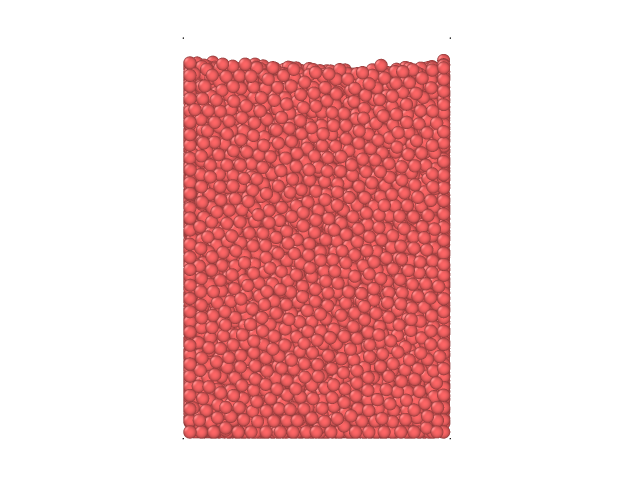
\includegraphics[width=\textwidth]{chapters/figures/heating_dte-02/15/0.15_pre_heat.png}
		\caption{Side-view of the pebble bed after resettling from the crushing event, before heating.}
		\label{fig:15percent-crushed-pre}
	\end{subfigure}
	\begin{subfigure}[t]{\doubleimagewidth}
		\centering
		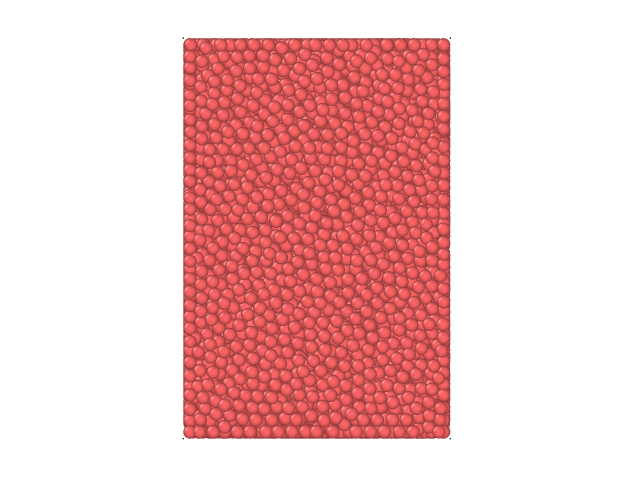
\includegraphics[width=\textwidth]{chapters/figures/heating_dte-02/15/0.15_post_heat.png}
		\caption{Side-view of the pebble bed after heating}
		\label{fig:15percent-crushed-swelling}
	\end{subfigure}
	\caption{In (a) we see the pebble bed after 15\% of the pebbles have been crushed (removed) and then after the heating cycle in (b). The gap formed after crushing is completely filled by swelling pebbles.}
\end{figure}





\FloatBarrier


\subsection{Conclusions}
\label{sec:dem-conclusions}
This first study established the power of DEM modeling and its use as a foundation for the later studies with augmentations of helium flow. I simulated a pebble bed with a specified fraction of the pebbles crushed during operation, then determined the repercussions of the missing pebbles as they affect the macroscopic property of effective thermal conductivity. I used the assumption of homogeneous, random locations of pebble failure to induce a failure routine without requiring external loads on the bed to actually induce the pebble crushing. After heating to a steady-state, an effective thermal conductivity was calculated for the pebble bed. The results show that large amounts of pebble failure correspond to large decreases in the conductive transport of energy through the pebble bed. The increase was due almost exclusively to a drop in the inter-particle forces which lead to a large increase in temperature differences between neighboring pebbles.

As the first step in the modeling effort, there were many simplifications that had to be made. I will explain here the shortcomings of the assumptions and simplifications of this study before drawing any major conclusions from the results.

First, the `container walls' surrounding the pebble bed in this model are completely rigid and do not react as the swelling pebble bed presses into them while heating. The confined thermal expansion leads to higher contact forces in the pebble bed than what may exist in reality. Furthermore, as pointed out in the results, the initial contact force is strongly dependent on the \textit{initial packing state} and the contact forces are the greatest determining factor in $\keff$ for a bed. The initial packing state of the bed in this study gave abnormally high initial contact forces and thus abnormally high initiall $\keff$. A different packing scheme was shown to result in the same initial packing fraction but with greatly reduced initial contact forces; this packing technique will be used in future models. 

Second, we saw from Fig.\ref{fig:temp-scatters} that the majority of the pebbles in the ensemble have their temperatures close fitting to an average curve but a number of the pebbles had less thermal contact with neighboring particles and consequently had much larger temperatures. This was true even in the baseline case of a tightly packed ($\phi =$\num{0.64}) pebble bed. This phenomena is possible because the contribution to heat transfer of the interstitial gas was not considered in this model and the flowing helium gas is expected to prevent any runaway temperatures of individual pebbles as it provides another route of energy transfer in the bed. This will be addressed in \cref{sec:cfd-dem-studies}.

Lastly, the pebble crushing did not conserve mass between pre- and post-crushing in the pebble beds. This is an issue we address in the fragmentation study of \cref{sec:fragmentation}. There was also no predictive tool used to determine when pebbles would crush based on their inter-particle contact forces. I simply allowed an arbitrary number of pebbles to remove from the system. A predictive tool may not have expected even 2\% of the pebbles to be damaged, much less the 15\% to which I pushed the pebble bed. The predictive tool is discussed in \cref{sec:failure-study} and will be applied to later models.

In spite of the limitations mentioned, it is still worth drawing conclusions from the results of this study. The results shown in Figs.~\ref{fig:contact-forces-scatter} and~\ref{fig:coord-scatter} demonstrate that the heat transfer through a pebble bed is simultaneously a function of both the coordination number and inter-particle contact forces. The average values of both of these parameters reduced as pebbles in the bed were crushed. But by far the most important factor appears to be the inter-particle contact force. Between the baseline case and the bed with 15\% damage, the average inter-particle forces drop by an entire order of magnitude. The $\keff$ follow suit with a decrease to 10\% of the original value. Interestingly, when a pebble bed has lower overall inter-particle contact forces such as what we see when pebbles are crushed, we would predict fewer pebbles are likely to break. This result implies that pebble breakage is self-dampening; as pebbles begin to break the ensemble quickly relaxes and avoids future pebble failure. So while in this study we induced failure up to $\eta = 15\%$ without a concern for predicting if such a large amount would break, such large values may not occur in real beds during operation of a fusion reactor. 

The most important conclusion to draw from the this DEM study is simply the usefulness of the DEM tools for opening a window into the micro-mechanical world of the pebble bed. The transient DEM simulations allowed us to explore the evolving packing structure and the manifestation of the packings into macroscopic properties such as the effective thermal conductivity. The DEM simulations revealed that some of the most negative effects nervously anticipated in the solid breeder did not emerge: bed detachment from the walls and bridge-jamming of regions to isolate groups of pebbles from heat transfer paths. There remain some features which must be addressed, but the DEM approach used in this dissertation has demonstrated its value as a tool for solid breeder designers. 












%%%%%%%%%%%%%%%%%%%%%%%%%%%%%%%%%%%%%%%%%%%%%%%%%%%%%%%%%%%%%%%%%%%%%%%%%%%%%%%%%%%%%%%%%%%%%%
\section{Dynamically coupled CFD-DEM Study on Effective Conductivity of Pebble Peds with Pebble Damage}\label{sec:cfd-dem-studies}

In this section I demonstrate the transient coupling between DEM models of particle conductive heat transfer and inter-particle contact forces with the helium models of volume-averaged conservation equations. Thermal models of the pebble beds of solid breeders for fusion reactors are incomplete without consideration of the helium purge gas and its interaction with the poorly conductive porous network of pebbles. The simulation setup, material parameters, results and important conclusions will be discussed.

\subsection{Modeling Setup, Boundary Conditions, and Coupling}\label{sec:cfd-dem-setup}
We begin with the same well-packed pebble bed set up in \cref{sec:dem-studies-effective-conductivity}. With the inclusion of helium, we only consider a single representative damaged bed, with $\eta = 10$\%. The random removal technique of inducing `damage' to the bed was again used (in the same manner as described in \cref{sec:dem-studies-effective-conductivity}). The intent is to deduce changes in thermophysical properties when helium is considered in the thermal transport network of the pebble bed -- and as a function of the morphological changes due to damaged pebbles.

The fluid domain is constructed to include an inlet and outlet region of fluid. The inlet region is 5 pebble diameters in length and the outlet is 30 pebble diameters. No-slip boundary conditions are enforced at the walls at the $x$-limits of the region. To match the DEM domain, periodic boundary conditions are used in the $y$-limits. The inlet face of the fluid is specified at a constant $\vec{v} = 0.05$~cm/s. The outlet face is specified with OpenFOAM's `inletOutlet' command with a given pressure. This boundary condition allows the inlet pressure to float to value that satisfies the specified inlet velocity and outlet pressure. The temperature is specified as a constant $T_w = 573$~K at the $x$-walls as well as the inlet condition. The outlet condition of the temperature field is similarly given to be `inletOutlet' with OpenFOAM.

The size of the CFD cells were chosen to be large enough to fit approximately 5 pebbles, for which the divided technique of computing void fraction is applicable (see \cref{sec:lag-eul-mapping}); the ratio of cell volume to particle volume was $V_\text{cell} / V_p = 7.46$. The helium, in this first model, used constant fluid properties. The values are given in Table~\ref{tab:cfd-properties}.

The Koch-Hill-Ladd drag model is employed in the style of Model B with an Archimedes pressure for buoyancy term. The terminology of these CFD coupling drag models is discussed in Ref.~\cite{Zhou2010}. The Nusselt number correlation of Li \& Mason is used for the scalar transport simulation of energy. OpenFOAM's dummy turbulence model (which is nothing more than a laminar model) is used.

An implicit time marching scheme is employed with a time step in the fluid domain of $\Delta t_f = 10^{-4}$ s. The small time step is not necessary to capture the fluid flow. The momentum equation is essentially not even transient as a steady-state laminar solution is achieved almost instantaneously in comparison to the long time span required to reach thermal steady state. The small time step is necessary for a relatively tight coupling to the pebble bed as the temperatures increase on the pebbles. Integration schemes of gradients, divergence terms, and laplacians are all Gauss linear or Gauss limitedLinear (as defined in OpenFOAM). The time step of the DEM is $\Delta t_f = 10^{-7}$ s which must be small for stability of the DEM explicit integration. The coupling between CFD and DEM domains occurs every 10 time steps of the fluid domain - equating to every 10000 in the pebble domain.

The layout of the pebble bed inside the CFD domain is shown in Figs.~\ref{fig:cfdem-domain-z}, \ref{fig:cfdem-domain-z}, and~\ref{fig:cfdem-domain-z}. Notable of the layout is how we relax the size of the meshes in the direction of the periodic boundaries. The size is permitted as there are few variations in fluid or temperature in the periodic direction. The meshes are made much smaller in the direction between cooling boundaries. In this direction ($x$-direction), we need the meshes small enough to resolve a temperature profile across the bed between centerline and cooling boundaries. We also want to capture the behavior of near-wall arrangement of the pebble bed. 

\begin {table}[htp] %
\caption{Constant fluid properties of helium purge gas in CFD-DEM coupling.}
\label {tab:cfd-properties} \centering %
\begin {tabular}{ ccccc }
\toprule %
$\nu$				&	$\alpha$				&	$k$		&	$C_p$		& $\rho$		\\
(m$^2$/s)			&	(m$^2$/s)				&	(W/m-K)	&	(J/kg-K)	& (kg/m$^3$)	\\\toprule
$4.02\times 10^{-4}$&	$6.06\times 10^{-4}$	& 	0.2		& 	5192.8		& 	0.175		\\\bottomrule
\end{tabular}
\end{table}


\begin{figure}[t]
	\centering
	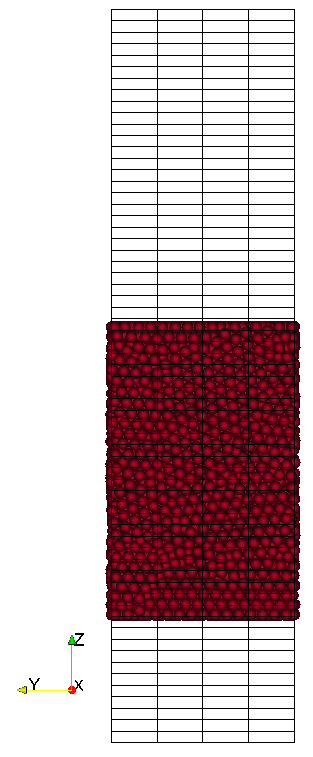
\includegraphics[width=0.4\textwidth]{chapters/figures/x-side-view}
    \caption{Side view of the pebble bed as it resides in the CFD mesh. The meshes in the direction of the periodic faces are allowed to be larger than others.}\label{fig:cfdem-domain-x}
\end{figure}

\begin{figure}[t]
	\centering
	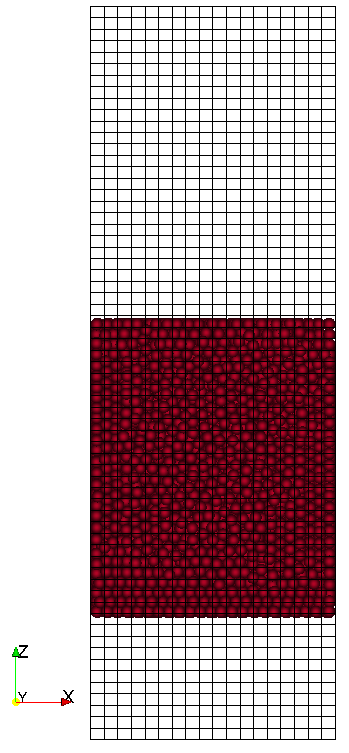
\includegraphics[width=0.4\textwidth]{chapters/figures/y-side-view}
    \caption{Front view of the pebble bed as it resides in the CFD mesh. The meshes in the direction of cooling are chosen to be large enough to fit many pebbles but small enough to provide a resolved temperature profile.}\label{fig:cfdem-domain-y}
\end{figure}

\begin{figure}[t]
	\centering
	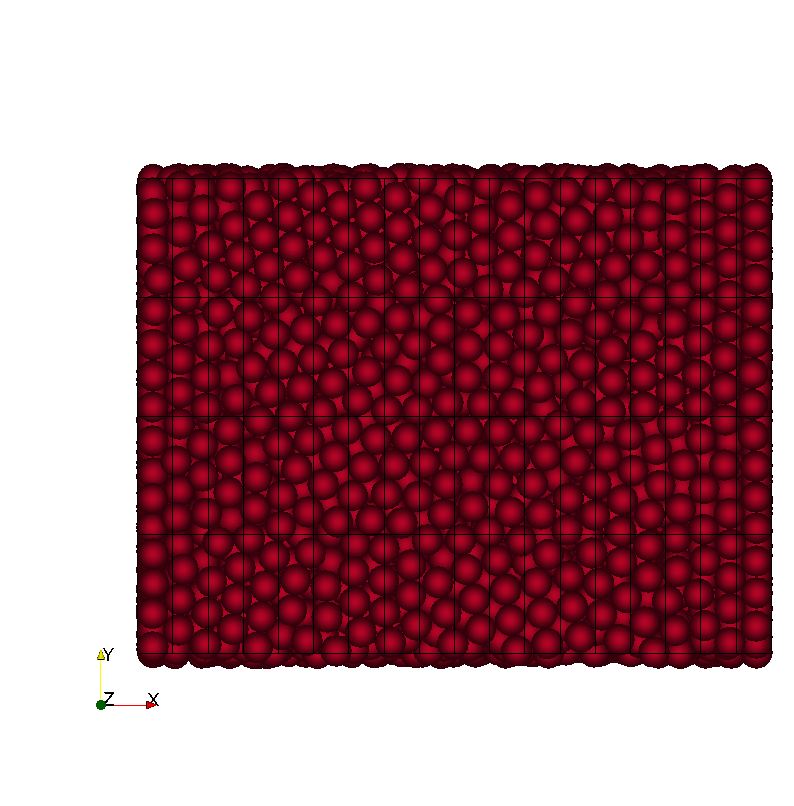
\includegraphics[width=\singleimagewidth]{chapters/figures/z-top-view}
    \caption{Top view of the pebble bed as it resides in the CFD mesh.}\label{fig:cfdem-domain-z}
\end{figure}


While the energy transport is the main concern of the pebble bed, we perform a simple validation of the CFD-DEM routine against known pressure-drop correlations to provide confidence in the overall coupling and volume-averaging technique. After pressure drop is shown to be consistent with empirical predictions, we can go through the thermal results.
\FloatBarrier
\section{Pressure Drop}
Before analyzing thermal results from the CFD-DEM coupling, the system was run at various particle Reynolds numbers and the overall pressure drop of the packed bed was measured. This value was compared against the well-known Kozeny-Carman and Ergun equations. The Kozeny-Carman is known to fit better with experimental data at very small Reynolds numbers. In Fig.~\ref{fig:cfdem-pressure-drop} we see the CFD-DEM coupling model is providing bed-scale pressure drops that match very well with Kozeny-Carman over the Reynold’s numbers applicable to helium purge flow in fusion reactors.

The flow is visualized in Fig.~\ref{fig:cfdem-streamlines}. The pebble bed is clipped at the centerline to allow viewing of the helium streamlines. Apparent in the figure is temperature profiles in the helium from centerline to wall that qualitatively mirror temperature profiles in the pebble bed.

\begin{figure}
        \centering
        \begin{subfigure}[b]{0.7\textwidth}
                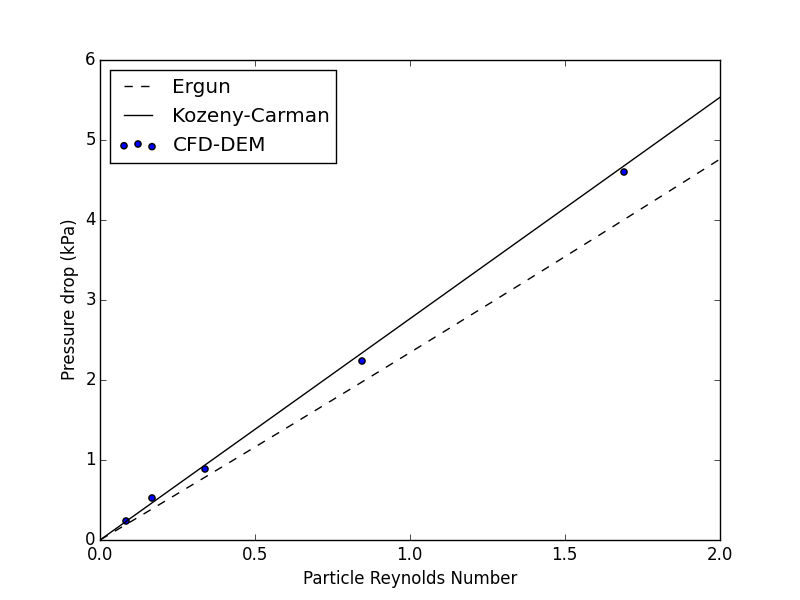
\includegraphics[width=\textwidth]{chapters/figures/pressureDrops-full.png}
                \caption{Well-packed bed}
                \label{fig:pressure-drop-full}
        \end{subfigure}%
        
          %add desired spacing between images, e. g. ~, \quad, \qquad, \hfill etc.
          %(or a blank line to force the subfigure onto a new line)
        \begin{subfigure}[b]{0.7\textwidth}
                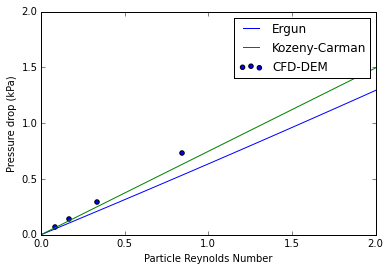
\includegraphics[width=\textwidth]{chapters/figures/pressureDrops-evap.png}
                \caption{Re-settled bed}
                \label{fig:pressure-drop-evap}
        \end{subfigure}
        \caption{Pressure drop calculations across packed beds, solved by CFD-DEM, fit well to the Kozeny-Carman empirical relation.}\label{fig:cfdem-pressure-drop}
\end{figure}



\begin{figure}[t]
	\centering
	\caption{Cut-away view of the pebble bed with streamlines of helium moving in generally straight paths from inlet to exit.}
	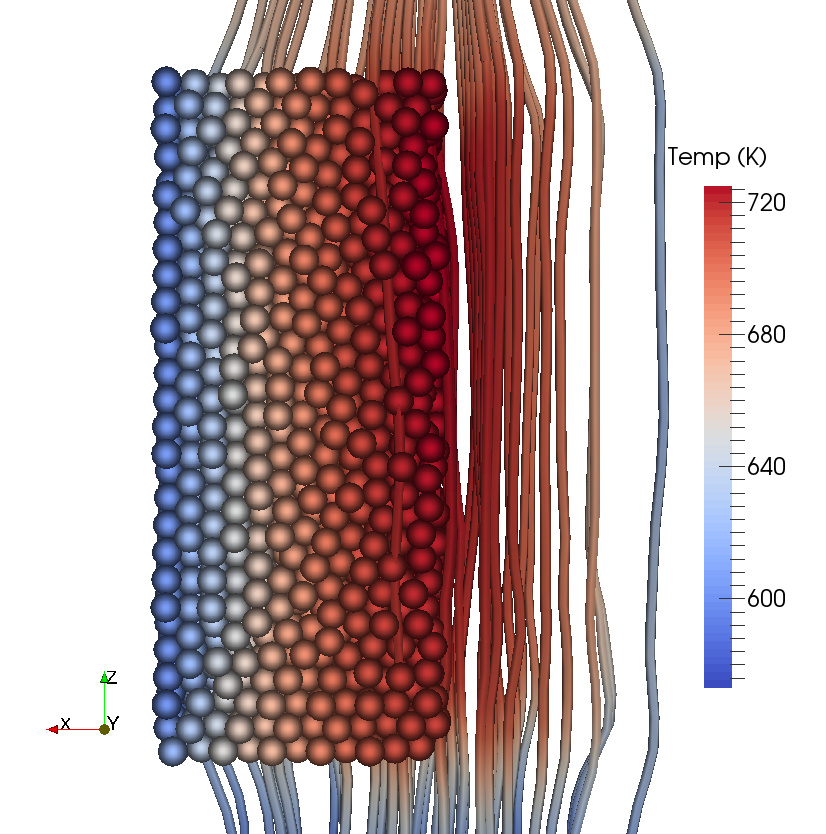
\includegraphics[width=0.75\textwidth]{chapters/figures/cfd-dem-streamlines2}\label{fig:cfdem-streamlines}
\end{figure}




\begin{figure}
        \centering
        \begin{subfigure}[b]{0.5\textwidth}
                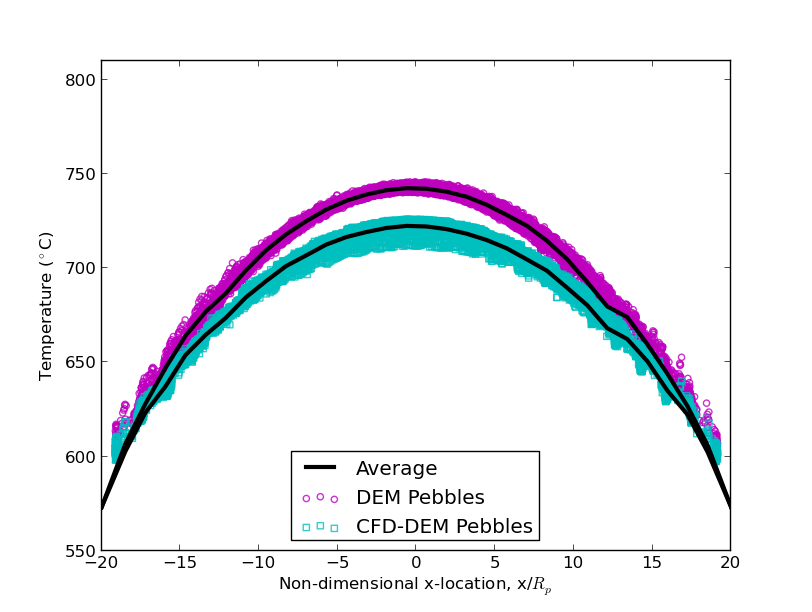
\includegraphics[width=\textwidth]{chapters/figures/full-x-T-color}
                \caption{Well-packed bed}
                \label{fig:x-T-full}
        \end{subfigure}%
        
          %add desired spacing between images, e. g. ~, \quad, \qquad, \hfill etc.
          %(or a blank line to force the subfigure onto a new line)
        \begin{subfigure}[b]{0.5\textwidth}
                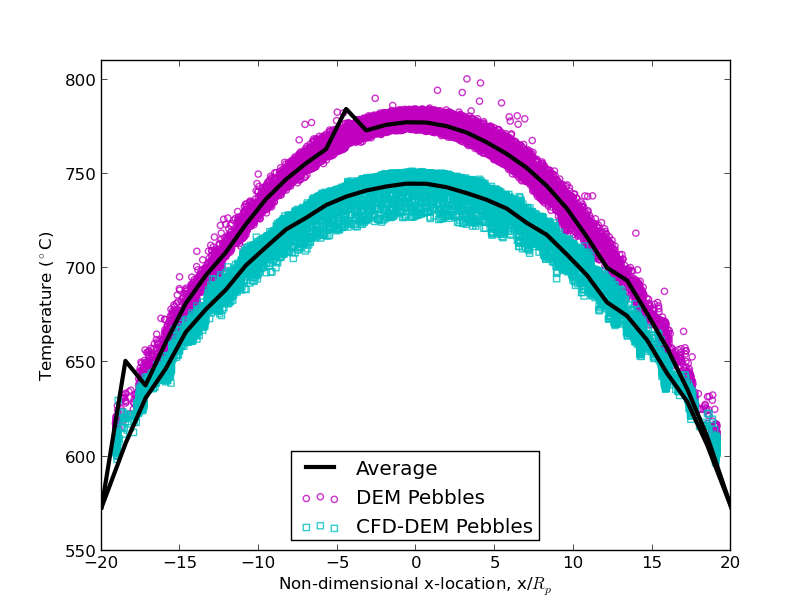
\includegraphics[width=\textwidth]{chapters/figures/evap-x-T-color}
                \caption{Re-settled bed}
                \label{fig:x-T-evap}
        \end{subfigure}
        \caption{Scatter temperature profiles of pebbles in a bed that is: well-packed (left) and resettled after 10\% of pebbles were removed from crushing (right). The introduction of helium into the simulation contributes to both lower overall temperatures (higher effective conductivity) and the smoothing out of high temperatures of isolated pebbles.}\label{fig:cfdem-x-T}
\end{figure}
\subsection{Effective Thermal Conductivity from CFD-DEM}\label{sec:cfd-dem-effective-conductivity}

The simulation is allowed to run to thermal steady-state with nuclear heating and wall cooling. After reaching a steady solution, I analyze the temperature profiles of the fluid and pebble bed. The temperature of the fluid volume from the simulation of the well-packed bed is shown in Fig.~\ref{fig:cfdem-complete-domain}. The flow field is also visualized in Fig.~\ref{fig:cfdem-streamlines}; in this figure the pebble bed is clipped at the centerline to allow viewing of the helium streamlines. Apparent in the figure is temperature profiles in the helium from centerline to wall that qualitatively mirror temperature profiles in the pebble bed. The two beds in our system, well-packed and resettled, were run to thermal steady-state with nuclear heating and wall cooling in both pure DEM and coupled CFD-DEM simulations for comparison. From steady-state temperature distributions, seen in the pebble scatter plots in Fig.~\ref{fig:cfdem-x-T}, an average profile is calculated and an effective thermal conductivity computed following the procedure shown in \cref{sec:keff-analogy}. The values are tabulated in Table~\ref{tab:cfdem-keff}. 

In the case of pure DEM, energy is transported solely along conduction routes in the ensemble. When the packing of the bed is disturbed, this results in a substantial drop in effective conductivity (a drop of 31\%). Perhaps more important than the reduction in effective conductivity, is the growth in number of isolated rattlers. Because heat deposition is volumetrically applied, pebbles with poor conduction routes become much hotter than their neighbors. This is evident in the high temperatures seen in many of the pebbles in the Fig.~\ref{fig:x-T-evap}. Over-heating of isolated pebbles could induce sintering and impact their tritium release even when the average temperatures measured in the bed are well below sintering values.

When CFD-DEM beds are analyzed, there is still a large reduction in effective conductivity (22\% drop), but interesting to note is the lack of high temperature rattlers. In the CFD-DEM scatter plot of Fig.~\ref{fig:x-T-evap}, there is evidence of the reduced heat transfer in the same region as the isolated pebbles from the DEM bed, but the temperatures are much closer to the average values of neighboring pebbles. The helium purge gas has locally smoothed out the temperatures and provided heat transport paths for pebbles that have loose physical contact with neighbors.

In spite of the 22\% decrease in effective conductivity, the maximum temperature of the pebble bed only increased 6.2\% (from \SIlist{725;751}{\kelvin} when helium is included in the model. This result is significant for solid breeder designers. They may choose a solid breeder volume such that in the event of extensive pebble cracking, the maximum temperature of the bed would remain within the ideal windows dictate for the lithium ceramics.

An accompanying result is the increased amount of energy carried out of the system by the helium purge gas. In Table I, the last column provides the ratio of energy carried out of the system to the nuclear energy deposited into the bed. The amount of energy carried out by the helium increased from \numlist{1.15;1.52}\% from the well-packed to damaged beds.

\begin{figure}[t]
    \centering
    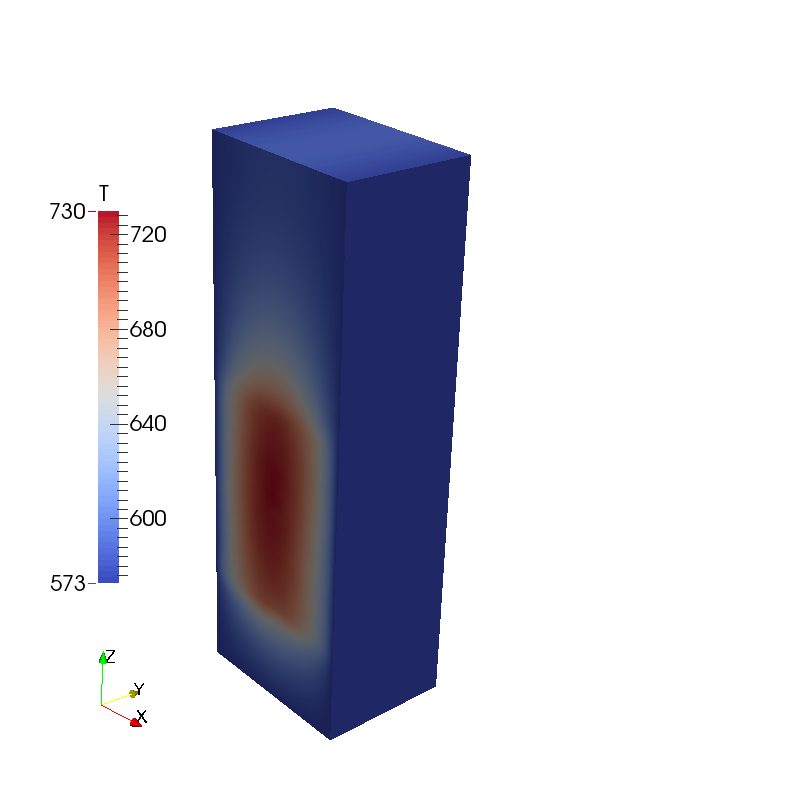
\includegraphics[width=\singleimagewidth]{chapters/figures/full-cfd-dem-fluid-temp}
    \caption{View of the complete fluid domain at thermal steady state.}\label{fig:cfdem-complete-domain}
\end{figure}


\begin{figure}[t]
    \centering
    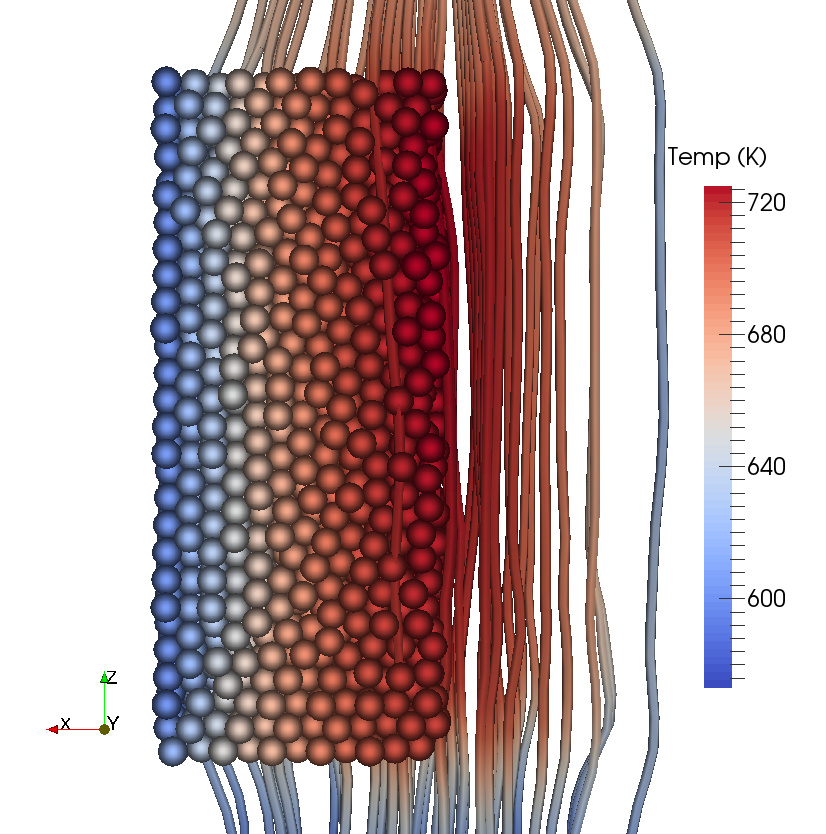
\includegraphics[width=\singleimagewidth]{chapters/figures/cfd-dem-streamlines2}
    \caption{Cut-away view of the pebble bed with streamlines of helium moving in generally straight paths from inlet to exit.}\label{fig:cfdem-streamlines}
\end{figure}


\begin{figure}
        \centering
        \begin{subfigure}[b]{0.5\textwidth}
                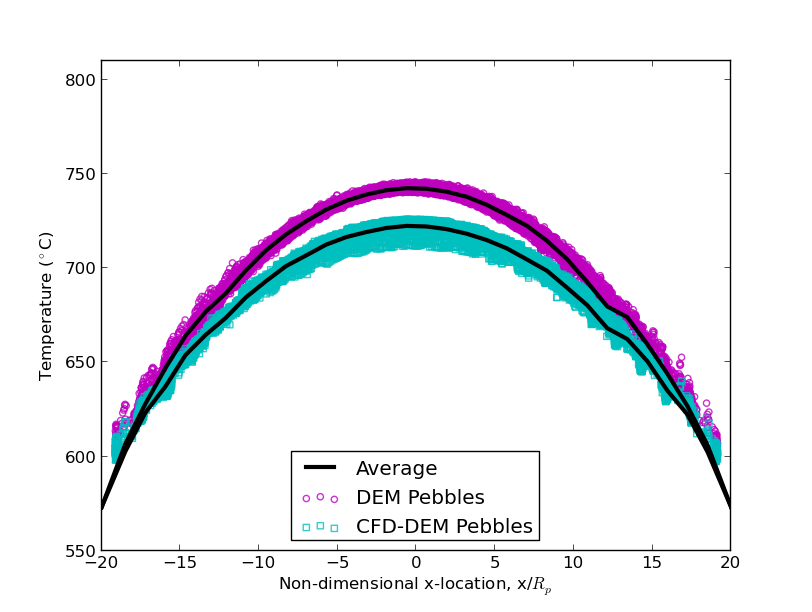
\includegraphics[width=\textwidth]{chapters/figures/full-x-T-color}
                \caption{Well-packed bed}
                \label{fig:x-T-full}
        \end{subfigure}%
        
          %add desired spacing between images, e. g. ~, \quad, \qquad, \hfill etc.
          %(or a blank line to force the subfigure onto a new line)
        \begin{subfigure}[b]{0.5\textwidth}
                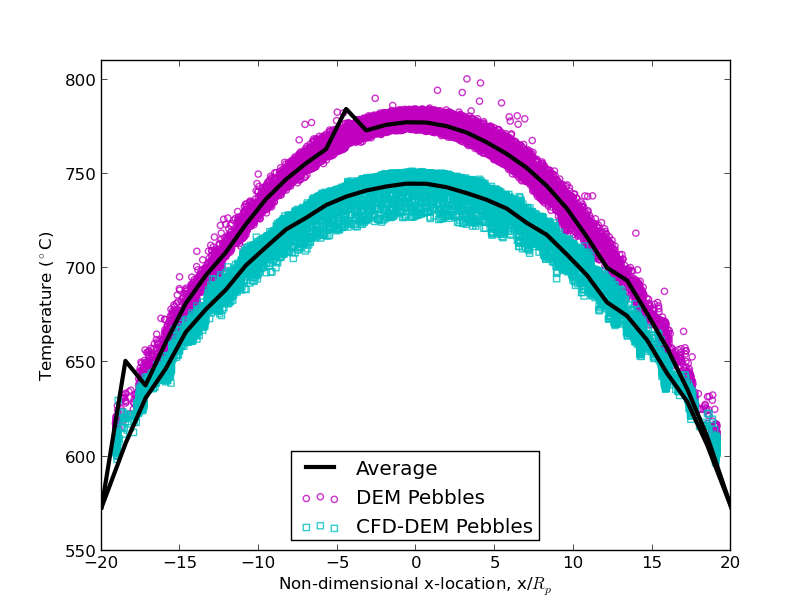
\includegraphics[width=\textwidth]{chapters/figures/evap-x-T-color}
                \caption{Re-settled bed}
                \label{fig:x-T-evap}
        \end{subfigure}
        \caption{Scatter temperature profiles of pebbles in a bed that is: well-packed (left) and resettled after 10\% of pebbles were removed from crushing (right). The introduction of helium into the simulation contributes to both lower overall temperatures (higher effective conductivity) and the smoothing out of high temperatures of isolated pebbles.}\label{fig:cfdem-x-T}
\end{figure}



\begin {table}[htp] %
\caption{Pebble bed values from the test matrix of the beds analyzed in this study.}
\label {tab:cfdem-keff} \centering %
\begin {tabular}{ rccccc }
\toprule %
			& 	\multicolumn{2}{c}{$\keff$}	&   \multicolumn{2}{c}{$T_\text{max}$}	&	$\frac{Q_h}{Q_\text{nuc}}$		\\
			& 	\multicolumn{2}{c}{(\si{\watt\per\meter\per\kelvin})}			&	\multicolumn{2}{c}{(\si{\kelvin})}				&									\\
			& 	DEM 		& 	CFD-DEM				&	DEM 		& 	CFD-DEM 			& 	CFD-DEM							\\\toprule
Well-packed	& 	0.96		& 	1.09				& 	745			& 	725					& 	1.15							\\
Resettled	& 	0.66		& 	0.85				& 	800			& 	751					& 	1.52							\\\bottomrule
\end{tabular}
\end{table}





\FloatBarrier



\subsection{Conclusions}

In this study I extended the thermophysical analysis of damaged pebble beds begun in \cref{sec:dem-studies} to include the influence of helium in a volume-average sense. This study grew from the prior one and the pebble bed representation of damage suffered all the same limitations mentioned in the closing of the last study, they will not be mentioned again here for the sake of brevity.

The CFD-DEM approach was validated, at least in terms of the volume-averaged Navier-Stokes equations, with a parametric study of pressure drop as a function of Reynolds number. When helium flowed over the DEM pebble beds, the pressure drop fit well to the well-established Kozeny-Carman correlation.

Two representative pebble beds, one well-packed and one with 10\% damaged pebbles, were run to thermal steady state with nuclear heating and cooling at a pair of walls.  The pair of pebble beds were considered with only conduction heat transfer of DEM and also with the helium enhancements to heat transfer with CFD-DEM. In the DEM beds, we saw that there always exist hot rattlers in pebble beds -- even well-packed ones. These pebbles heat from the volumetric source but have no outlet for the energy as their contacts with neighbors are very light. However, with the inclusion of helium flow eliminated the hot rattlers from both pebble beds analyzed.

When comparing the impact of pebble damage with and without the modeling of helium, the models including helium showed less of an impact on reduced effective thermal conductivity when the bed experienced the extensive 10\% damage of pebbles. Furthermore, the maximum bed temperature increased less due to pebble damage when helium was included, when compared to DEM-only beds.

This study is a useful demonstration of the power of the dynamically coupled CFD-DEM approach. The DEM simulation was capable of continually monitoring inter-particle forces and individual particle temperatures such that any of the crush-prediction, fragmentation, and thermal expansion methods developed in this dissertation can continue to transiently alter the morphology of the pebble bed. Meanwhile, the volume-averaged approach to conservation equations of the fluid allow for an efficient overlaying of the fluid contribution to the thermophysical behavior of the pebble bed.

There are simplifications to the fluid flow and its impact on the thermal transport in the pebble bed that are made in the volume-averaging technique. The simplifications may mask some important physical features of the flow and energy fields but nevertheless provide valuable information on the pebble bed in an efficient manner and should continue to be developed for solid breeder research.



%%%%%%%%%%%%%%%%%%%%%%%%%%%%%%%%%%%%%%%%%%%%%%%%%%%%%%%%%%%%%%%%%%%%%%%%%%%%%%%%%%%%%%%%%%%%%%
\section{3D Lattice-Boltzmann Models of the Complete Conjugate Heat Transfer of Helium Purge Gas and Ceramic Pebble Beds}\label{sec:lbm-studies}

In this section I apply the lattice-Boltzmann numerical modeling tools to study the complete interstitial flow of helium through a packed bed of lithium ceramics. Pebble packing structures are developed with the same DEM simulations that lead to packings input into the CFD-DEM demonstration study. However, instead of the fluid modeling dynamically coupling to DEM models of the evolving packing structure, I map snapshots of the DEM pebble bed into the LBM nodal grids. Once in LBM, the helium flow and thermal interaction between fluid and solid and internally in solid are fully modeled with lattice dynamics defined in the LBM framework. The LBM approach sacrifices dynamic coupling for complete models of the tortuous flow. Details of the lattice parameters and results of the simulation are provided.

\subsection{Model Setup \& Methodology}

Based on the discussion of \cref{sec:physical-to-lattice}, all we need to specify our simulation is the resolution (number of nodes per pebble diameter) and time step size. For this simulation we choose a resolution of $\text{res} = 10$ and a time step of $\delta_t = 0.001$. The rest of the descriptions of our pebble bed are locked from the system and material properties. The geometric values for the lattice are given in Table~\ref{tab:lbm-parameters}, the relaxation parameters defining the collision dynamics of the lattices are given in Table~\ref{tab:lbm-relaxations}, and the boundary conditions are given in Table~\ref{tab:lbm-boundaries}. The values are all unitless in the lattice framework and are translated from the physical values to match the model of \cref{sec:cfd-dem-studies}

\begin {table}[htp] %
\caption{Physical description of the lattice (in lattice units).}
\label{tab:lbm-parameters} \centering %
\begin {tabular}{ cccccc }
\toprule %
$X^*$   &   $Y^*$  &   $Z^*$    &   res  & $\delta_x$   & $\delta_t$    \\\toprule
25      &   15     &   94.5     &   10   &  0.1         &  0.001        \\\bottomrule
\end{tabular}
\end{table}

\begin {table}[htp] %
\caption{The momentum relaxation time for fluid (ns), thermal relaxation time for fluid (ad), and thermal relaxation time for the solid (cj) used in the simulation.}
\label{tab:lbm-relaxations} \centering %
\begin {tabular}{ cccccccc }
\toprule %
$\tau_{ns}$ &  $\tau_{ad}$  &   $\tau_{cj}$     \\\toprule
0.7204      &  0.4375       &   0.9663          \\\bottomrule
\end{tabular}
\end{table}

\begin {table}[htp] %
\caption{Boundary conditions translated into lattice units.}
\label{tab:lbm-boundaries} \centering %
\begin {tabular}{ cccccccc }
\toprule %
$\vec{u}_\text{inlet}$    &  $T_\text{inlet}$   &  $T_\text{wall}$     \\\toprule
(0.005, 0, 0)           &  131.79           &   131.79          \\\bottomrule
\end{tabular}
\end{table}


The physical properties of helium from \cref{sec:cfd-dem-setup} are used here to calculate the relaxation time, $\tau_{ns}$ as outlined in \cref{sec:physical-to-lattice}. The physical description of the pebble bed analyzed with LBM is identical to the beds described in \cref{sec:cfd-dem-studies}. The details for mapping from our DEM packing to the LBM lattice are given in \cref{sec:dem2lbm-mapping}. With the mechanisms described there we can define the lattice nodes definitions (being either solid or fluid) simply with specifying the resolution.

When running the simulation, the lattice running the collision and streaming of the Navier-Stokes density distribution functions would consistently return a stable and steady fluid velocity after the initial oscillations from the initial conditions. Unfortunately, at this point, the thermal lattice will run smoothly until a certain time when an instability at the outlet propagates upstream and destroys the results of the entire thermal lattice. These preliminary results will therefore focus on the velocity results and the initial thermal results (it would not reach thermal steady-state before crashing). Even with this caveat on the results, what we do see from the LBM results are extremely encouraging for the use of the method in the future.






\subsection{Laminar Mixing of Energy in Packed Beds with Volumetric Heating}

It is well known that a fluid moving through a packed bed will follow a path much longer than the length of the packed bed. The extended path is often reported as the tortuosity of the packed bed. In the ceramic breeder packed beds for tritium generation, the tortuosity of the helium flow modeled in LB resulted in 

% \begin{figure}[t]
%     \centering
%     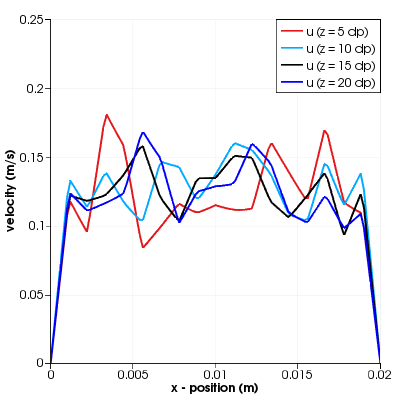
\includegraphics[width=\singleimagewidth]{chapters/figures/lbm/evap-u-profiles}
%     \caption{Velocity profiles (in the $x$-direction) at varying pebble bed heights for the pebble bed with 10\% damaged pebbles.}\label{fig:lbm-evap-u-profile}
% \end{figure}

\begin{figure}[t]
    \centering
    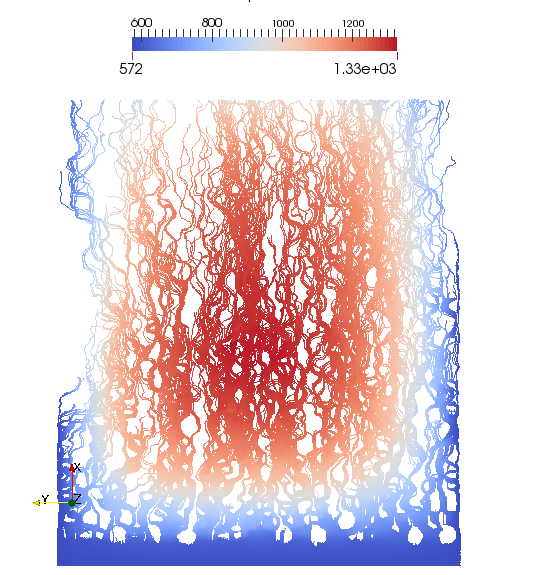
\includegraphics[width=\singleimagewidth]{chapters/figures/lbm/lbm-streamlines}
    \caption{Demonstrating the meandering path -- importantly wandering in the $x$-direction -- of fluid flow in the pebble bed.}\label{fig:lbm-streamlines}
\end{figure}

\begin{figure}[t]
    \centering
    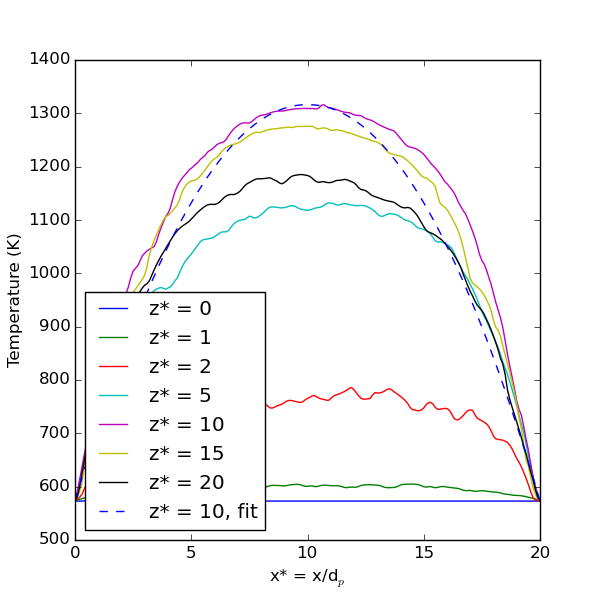
\includegraphics[width=\singleimagewidth]{chapters/figures/lbm/lbm-temp-profiles}
    \caption{Temperature profiles (in the $x$-direction) at varying pebble bed heights for the pebble bed with 10\% damaged pebbles. Shown for comparison is a parabolic profile that had fit both DEM and CFD-DEM temperature results.}\label{fig:lbm-temp-profiles}
\end{figure}

\begin{figure}[t]
    \centering
    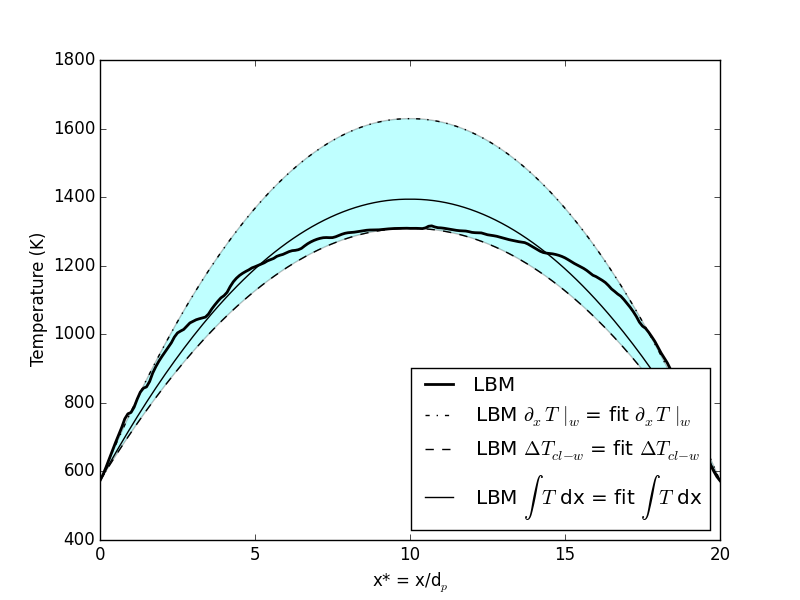
\includegraphics[width=\singleimagewidth]{chapters/figures/lbm/lbm-temp-profile_parabolic}
    \caption{Temperature profile from the LBM model is bound by parabolic curves. The LBM temperature profile increases sharply near the wall but then is flattened near the centerline. The behavior is indicative of laminar mixing of energy in the bed.}\label{fig:lbm-temp-parabolas}
\end{figure}

\begin{figure}[t]
    \centering
    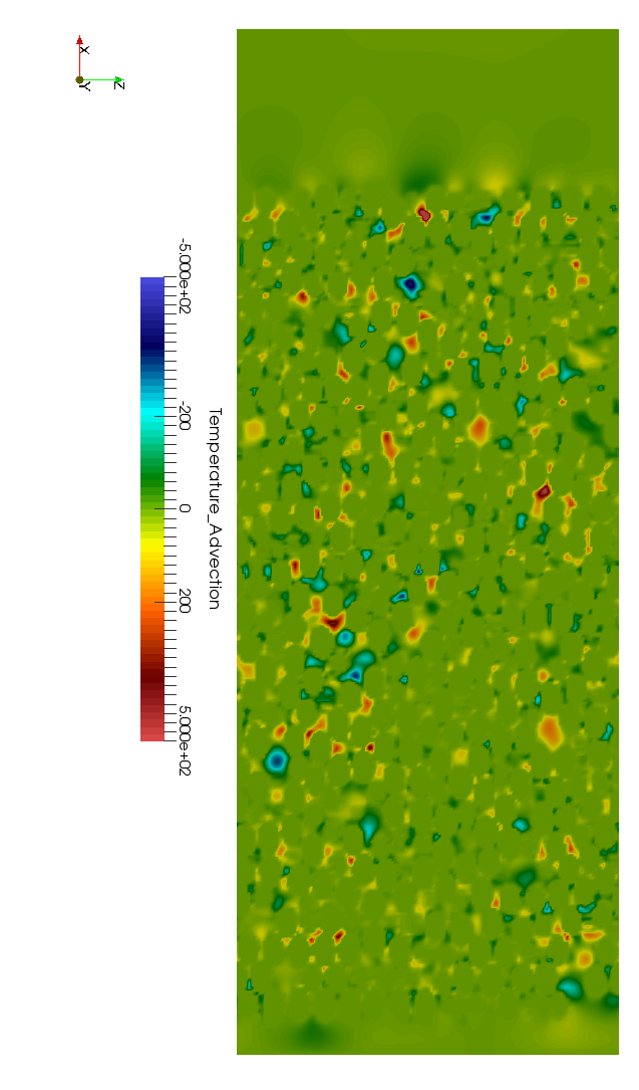
\includegraphics[width=\singleimagewidth]{chapters/figures/lbm/lbm-laminar-mixing}
    \caption{Slice of LBM simulation.}\label{fig:lbm-laminar-mixing}
\end{figure}

\FloatBarrier

\subsection{Conclusions}







%%%%%%%%%%%%%%%%%%%%%%%%%%%%%%%%%%%%%%%%%%%%%%%%%%%%%%%%%%%%%%%%%%%%%%%%%%%%%%%%%%%%%%%%%%%%%%
\section{Summary, Discussion, \& Conclusions}

I showcased the three numerical tools developed for analyzing pebble-scale micro-mechanics in ceramic pebble beds for solid breeders. The three studies demonstrated the effectiveness of the code to present information on the physics dictating heat transfer and force balance inside pebble beds. The conduction heat transfer in the bed was seen to be tightly dependent on the morphology of the packed bed - more complicated than the common descriptor of packing fraction. The single largest factor determining effective conductivity (in a pure conduction environment) is the normal forces in the contact force network of a bed. When the pebbles were modeled as broken and removed from the system, an increased fraction of the pebbles became hot rattlers which were much hotter than their neighboring pebbles. 

The size and complexity of porous beds make it impractical for modeling conjugate heat transfer on pebble-scale with conventional CFD tools, I therefore introduced two efficient methods for modeling helium purge gas interacting with packed beds: 1) directly coupled CFD-DEM for volume-averaged fluid-pebble and discrete pebble-pebble interactions and 2) DEM packing structures imported into LBM simulations for more detailed modeling of fluid flow and thermal transport. After incorporation of helium into the thermal model, the isolated pebbles witnessed in the DEM heat transfer simulation had their temperatures equilibrate more readily with their local region; hot spots seen in DEM models essentially disappeared in both models which included helium flow. Finally, in the lattice-Boltzmann simulation, the heat transfer between the center of the bed toward the cooling walls was influenced strongly by even the slow tortuous flow of helium in that direction - a phenomena referred to as laminar mixing of energy.

For a homogeneously packed bed, it is common practice to assign an effective thermal conductivity to the entire volume. Even in experiments measuring the effective thermal conductivity of a pebble bed in a helium environment, a constant value of $\keff$ is observed. The impact of laminar mixing will not emerge until the system has the specific characteristics of the fusion reaction, most importantly: volumetric heating and flowing helium. It is only in the combination of transverse flow in the direction of cooling that the phenomena arises. The effect of laminar mixing was seen to push the temperature profile of the packed bed away from the parabola defined by a constant effective thermal conductivity. Very advantageously, the maximum temperature in the flowing helium pebble bed is lowered and the temperature near the walls is increased as compared to a constant $\keff$ computation.

The design margins of ceramic solid breeders is, in fact, quite narrow. The requirement on bed temperatures to be below the sintering temperature of the ceramic, in conjunction with low thermal conductivity of the bed, constricts the size of the power density allowable to bombard the lithium ceramic. Furthermore, the temperature-dependence of tritium release in the ceramic pushes them toward ideally operating in as high of temperature regimes as possible. The laminar mixing described in the pebble bed works to benefit both of the temperature requirements described here: lower maximum temperature for higher power density and higher near-wall temperatures for increased tritium release rates.









\end{document}






